\documentclass[twoside]{book}

% Packages required by doxygen
\usepackage{fixltx2e}
\usepackage{calc}
\usepackage{doxygen}
\usepackage[export]{adjustbox} % also loads graphicx
\usepackage{graphicx}
\usepackage[utf8]{inputenc}
\usepackage{makeidx}
\usepackage{multicol}
\usepackage{multirow}
\PassOptionsToPackage{warn}{textcomp}
\usepackage{textcomp}
\usepackage[nointegrals]{wasysym}
\usepackage[table]{xcolor}

% Font selection
\usepackage[T1]{fontenc}
\usepackage[scaled=.90]{helvet}
\usepackage{courier}
\usepackage{amssymb}
\usepackage{sectsty}
\renewcommand{\familydefault}{\sfdefault}
\allsectionsfont{%
  \fontseries{bc}\selectfont%
  \color{darkgray}%
}
\renewcommand{\DoxyLabelFont}{%
  \fontseries{bc}\selectfont%
  \color{darkgray}%
}
\newcommand{\+}{\discretionary{\mbox{\scriptsize$\hookleftarrow$}}{}{}}

% Page & text layout
\usepackage{geometry}
\geometry{%
  a4paper,%
  top=2.5cm,%
  bottom=2.5cm,%
  left=2.5cm,%
  right=2.5cm%
}
\tolerance=750
\hfuzz=15pt
\hbadness=750
\setlength{\emergencystretch}{15pt}
\setlength{\parindent}{0cm}
\setlength{\parskip}{3ex plus 2ex minus 2ex}
\makeatletter
\renewcommand{\paragraph}{%
  \@startsection{paragraph}{4}{0ex}{-1.0ex}{1.0ex}{%
    \normalfont\normalsize\bfseries\SS@parafont%
  }%
}
\renewcommand{\subparagraph}{%
  \@startsection{subparagraph}{5}{0ex}{-1.0ex}{1.0ex}{%
    \normalfont\normalsize\bfseries\SS@subparafont%
  }%
}
\makeatother

% Headers & footers
\usepackage{fancyhdr}
\pagestyle{fancyplain}
\fancyhead[LE]{\fancyplain{}{\bfseries\thepage}}
\fancyhead[CE]{\fancyplain{}{}}
\fancyhead[RE]{\fancyplain{}{\bfseries\leftmark}}
\fancyhead[LO]{\fancyplain{}{\bfseries\rightmark}}
\fancyhead[CO]{\fancyplain{}{}}
\fancyhead[RO]{\fancyplain{}{\bfseries\thepage}}
\fancyfoot[LE]{\fancyplain{}{}}
\fancyfoot[CE]{\fancyplain{}{}}
\fancyfoot[RE]{\fancyplain{}{\bfseries\scriptsize Generated by Doxygen }}
\fancyfoot[LO]{\fancyplain{}{\bfseries\scriptsize Generated by Doxygen }}
\fancyfoot[CO]{\fancyplain{}{}}
\fancyfoot[RO]{\fancyplain{}{}}
\renewcommand{\footrulewidth}{0.4pt}
\renewcommand{\chaptermark}[1]{%
  \markboth{#1}{}%
}
\renewcommand{\sectionmark}[1]{%
  \markright{\thesection\ #1}%
}

% Indices & bibliography
\usepackage{natbib}
\usepackage[titles]{tocloft}
\setcounter{tocdepth}{3}
\setcounter{secnumdepth}{5}
\makeindex

% Hyperlinks (required, but should be loaded last)
\usepackage{ifpdf}
\ifpdf
  \usepackage[pdftex,pagebackref=true]{hyperref}
\else
  \usepackage[ps2pdf,pagebackref=true]{hyperref}
\fi
\hypersetup{%
  colorlinks=true,%
  linkcolor=blue,%
  citecolor=blue,%
  unicode%
}

% Custom commands
\newcommand{\clearemptydoublepage}{%
  \newpage{\pagestyle{empty}\cleardoublepage}%
}

\usepackage{caption}
\captionsetup{labelsep=space,justification=centering,font={bf},singlelinecheck=off,skip=4pt,position=top}

%===== C O N T E N T S =====

\begin{document}

% Titlepage & ToC
\hypersetup{pageanchor=false,
             bookmarksnumbered=true,
             pdfencoding=unicode
            }
\pagenumbering{alph}
\begin{titlepage}
\vspace*{7cm}
\begin{center}%
{\Large Simulation Visualization }\\
\vspace*{1cm}
{\large Generated by Doxygen 1.8.14}\\
\end{center}
\end{titlepage}
\clearemptydoublepage
\pagenumbering{roman}
\tableofcontents
\clearemptydoublepage
\pagenumbering{arabic}
\hypersetup{pageanchor=true}

%--- Begin generated contents ---
\chapter{Namespace Index}
\section{Namespace List}
Here is a list of all namespaces with brief descriptions\+:\begin{DoxyCompactList}
\item\contentsline{section}{\mbox{\hyperlink{namespaceec}{ec}} }{\pageref{namespaceec}}{}
\item\contentsline{section}{\mbox{\hyperlink{namespacer3}{r3}} }{\pageref{namespacer3}}{}
\end{DoxyCompactList}

\chapter{Hierarchical Index}
\section{Class Hierarchy}
This inheritance list is sorted roughly, but not completely, alphabetically\+:\begin{DoxyCompactList}
\item \contentsline{section}{Particle\+Node}{\pageref{class_particle_node}}{}
\item \contentsline{section}{Particle\+Node\+World}{\pageref{class_particle_node_world}}{}
\item \contentsline{section}{Physics\+Engine\+Wrapper}{\pageref{class_physics_engine_wrapper}}{}
\item \contentsline{section}{Rigid\+Body\+Node}{\pageref{class_rigid_body_node}}{}
\item \contentsline{section}{Rigid\+Body\+Node\+World}{\pageref{class_rigid_body_node_world}}{}
\item Scene\begin{DoxyCompactList}
\item \contentsline{section}{Simulation\+Scene}{\pageref{class_simulation_scene}}{}
\begin{DoxyCompactList}
\item \contentsline{section}{Falling\+Cube\+Scene}{\pageref{class_falling_cube_scene}}{}
\end{DoxyCompactList}
\end{DoxyCompactList}
\item Window\begin{DoxyCompactList}
\item \contentsline{section}{Simulation\+Window}{\pageref{class_simulation_window}}{}
\end{DoxyCompactList}
\end{DoxyCompactList}

\chapter{Class Index}
\section{Class List}
Here are the classes, structs, unions and interfaces with brief descriptions\+:\begin{DoxyCompactList}
\item\contentsline{section}{\mbox{\hyperlink{class_falling_cube_scene}{Falling\+Cube\+Scene}} }{\pageref{class_falling_cube_scene}}{}
\item\contentsline{section}{\mbox{\hyperlink{class_particle_node}{Particle\+Node}} }{\pageref{class_particle_node}}{}
\item\contentsline{section}{\mbox{\hyperlink{class_particle_node_world}{Particle\+Node\+World}} }{\pageref{class_particle_node_world}}{}
\item\contentsline{section}{\mbox{\hyperlink{class_physics_engine_wrapper}{Physics\+Engine\+Wrapper}} }{\pageref{class_physics_engine_wrapper}}{}
\item\contentsline{section}{\mbox{\hyperlink{class_rigid_body_node}{Rigid\+Body\+Node}} }{\pageref{class_rigid_body_node}}{}
\item\contentsline{section}{\mbox{\hyperlink{class_rigid_body_node_world}{Rigid\+Body\+Node\+World}} }{\pageref{class_rigid_body_node_world}}{}
\item\contentsline{section}{\mbox{\hyperlink{class_simulation_scene}{Simulation\+Scene}} }{\pageref{class_simulation_scene}}{}
\item\contentsline{section}{\mbox{\hyperlink{class_simulation_window}{Simulation\+Window}} }{\pageref{class_simulation_window}}{}
\end{DoxyCompactList}

\chapter{File Index}
\section{File List}
Here is a list of all files with brief descriptions\+:\begin{DoxyCompactList}
\item\contentsline{section}{D\+:/\+Library/\+Documents/\+Job/\+Forschungsmaster/\+Projekte/\+Simulation\+Visualization/\+Sim/\+Sim/src/\mbox{\hyperlink{main_8cpp}{main.\+cpp}} }{\pageref{main_8cpp}}{}
\item\contentsline{section}{D\+:/\+Library/\+Documents/\+Job/\+Forschungsmaster/\+Projekte/\+Simulation\+Visualization/\+Sim/\+Sim/src/\mbox{\hyperlink{_simulation_scene_8cpp}{Simulation\+Scene.\+cpp}} }{\pageref{_simulation_scene_8cpp}}{}
\item\contentsline{section}{D\+:/\+Library/\+Documents/\+Job/\+Forschungsmaster/\+Projekte/\+Simulation\+Visualization/\+Sim/\+Sim/src/\mbox{\hyperlink{_simulation_scene_8h}{Simulation\+Scene.\+h}} }{\pageref{_simulation_scene_8h}}{}
\item\contentsline{section}{D\+:/\+Library/\+Documents/\+Job/\+Forschungsmaster/\+Projekte/\+Simulation\+Visualization/\+Sim/\+Sim/src/\mbox{\hyperlink{_simulation_window_8cpp}{Simulation\+Window.\+cpp}} }{\pageref{_simulation_window_8cpp}}{}
\item\contentsline{section}{D\+:/\+Library/\+Documents/\+Job/\+Forschungsmaster/\+Projekte/\+Simulation\+Visualization/\+Sim/\+Sim/src/\mbox{\hyperlink{_simulation_window_8h}{Simulation\+Window.\+h}} }{\pageref{_simulation_window_8h}}{}
\item\contentsline{section}{D\+:/\+Library/\+Documents/\+Job/\+Forschungsmaster/\+Projekte/\+Simulation\+Visualization/\+Sim/\+Sim/src/\+Examples/\mbox{\hyperlink{_falling_cube_scene_8cpp}{Falling\+Cube\+Scene.\+cpp}} }{\pageref{_falling_cube_scene_8cpp}}{}
\item\contentsline{section}{D\+:/\+Library/\+Documents/\+Job/\+Forschungsmaster/\+Projekte/\+Simulation\+Visualization/\+Sim/\+Sim/src/\+Examples/\mbox{\hyperlink{_falling_cube_scene_8h}{Falling\+Cube\+Scene.\+h}} }{\pageref{_falling_cube_scene_8h}}{}
\item\contentsline{section}{D\+:/\+Library/\+Documents/\+Job/\+Forschungsmaster/\+Projekte/\+Simulation\+Visualization/\+Sim/\+Sim/src/\+Physic\+Interfaces/\mbox{\hyperlink{_particle_node_8cpp}{Particle\+Node.\+cpp}} }{\pageref{_particle_node_8cpp}}{}
\item\contentsline{section}{D\+:/\+Library/\+Documents/\+Job/\+Forschungsmaster/\+Projekte/\+Simulation\+Visualization/\+Sim/\+Sim/src/\+Physic\+Interfaces/\mbox{\hyperlink{_particle_node_8h}{Particle\+Node.\+h}} }{\pageref{_particle_node_8h}}{}
\item\contentsline{section}{D\+:/\+Library/\+Documents/\+Job/\+Forschungsmaster/\+Projekte/\+Simulation\+Visualization/\+Sim/\+Sim/src/\+Physic\+Interfaces/\mbox{\hyperlink{_particle_node_world_8cpp}{Particle\+Node\+World.\+cpp}} }{\pageref{_particle_node_world_8cpp}}{}
\item\contentsline{section}{D\+:/\+Library/\+Documents/\+Job/\+Forschungsmaster/\+Projekte/\+Simulation\+Visualization/\+Sim/\+Sim/src/\+Physic\+Interfaces/\mbox{\hyperlink{_particle_node_world_8h}{Particle\+Node\+World.\+h}} }{\pageref{_particle_node_world_8h}}{}
\item\contentsline{section}{D\+:/\+Library/\+Documents/\+Job/\+Forschungsmaster/\+Projekte/\+Simulation\+Visualization/\+Sim/\+Sim/src/\+Physic\+Interfaces/\mbox{\hyperlink{_physics_engine_wrapper_8cpp}{Physics\+Engine\+Wrapper.\+cpp}} }{\pageref{_physics_engine_wrapper_8cpp}}{}
\item\contentsline{section}{D\+:/\+Library/\+Documents/\+Job/\+Forschungsmaster/\+Projekte/\+Simulation\+Visualization/\+Sim/\+Sim/src/\+Physic\+Interfaces/\mbox{\hyperlink{_physics_engine_wrapper_8h}{Physics\+Engine\+Wrapper.\+h}} }{\pageref{_physics_engine_wrapper_8h}}{}
\item\contentsline{section}{D\+:/\+Library/\+Documents/\+Job/\+Forschungsmaster/\+Projekte/\+Simulation\+Visualization/\+Sim/\+Sim/src/\+Physic\+Interfaces/\mbox{\hyperlink{_rigid_body_node_8cpp}{Rigid\+Body\+Node.\+cpp}} }{\pageref{_rigid_body_node_8cpp}}{}
\item\contentsline{section}{D\+:/\+Library/\+Documents/\+Job/\+Forschungsmaster/\+Projekte/\+Simulation\+Visualization/\+Sim/\+Sim/src/\+Physic\+Interfaces/\mbox{\hyperlink{_rigid_body_node_8h}{Rigid\+Body\+Node.\+h}} }{\pageref{_rigid_body_node_8h}}{}
\item\contentsline{section}{D\+:/\+Library/\+Documents/\+Job/\+Forschungsmaster/\+Projekte/\+Simulation\+Visualization/\+Sim/\+Sim/src/\+Physic\+Interfaces/\mbox{\hyperlink{_rigid_body_node_world_8cpp}{Rigid\+Body\+Node\+World.\+cpp}} }{\pageref{_rigid_body_node_world_8cpp}}{}
\item\contentsline{section}{D\+:/\+Library/\+Documents/\+Job/\+Forschungsmaster/\+Projekte/\+Simulation\+Visualization/\+Sim/\+Sim/src/\+Physic\+Interfaces/\mbox{\hyperlink{_rigid_body_node_world_8h}{Rigid\+Body\+Node\+World.\+h}} }{\pageref{_rigid_body_node_world_8h}}{}
\end{DoxyCompactList}

\chapter{Namespace Documentation}
\hypertarget{namespaceec}{}\section{ec Namespace Reference}
\label{namespaceec}\index{ec@{ec}}

\hypertarget{namespacer3}{}\section{r3 Namespace Reference}
\label{namespacer3}\index{r3@{r3}}

\chapter{Class Documentation}
\hypertarget{class_falling_cube_scene}{}\section{Falling\+Cube\+Scene Class Reference}
\label{class_falling_cube_scene}\index{Falling\+Cube\+Scene@{Falling\+Cube\+Scene}}


{\ttfamily \#include $<$Falling\+Cube\+Scene.\+h$>$}



Inheritance diagram for Falling\+Cube\+Scene\+:\nopagebreak
\begin{figure}[H]
\begin{center}
\leavevmode
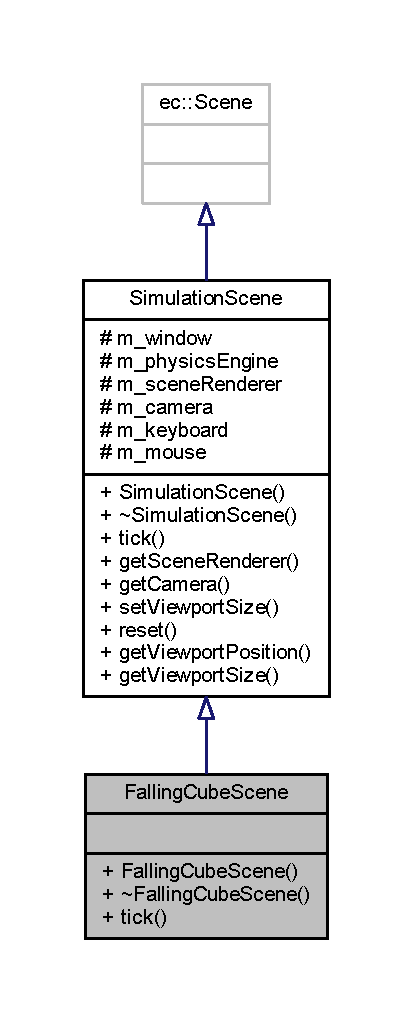
\includegraphics[width=198pt]{class_falling_cube_scene__inherit__graph}
\end{center}
\end{figure}


Collaboration diagram for Falling\+Cube\+Scene\+:\nopagebreak
\begin{figure}[H]
\begin{center}
\leavevmode
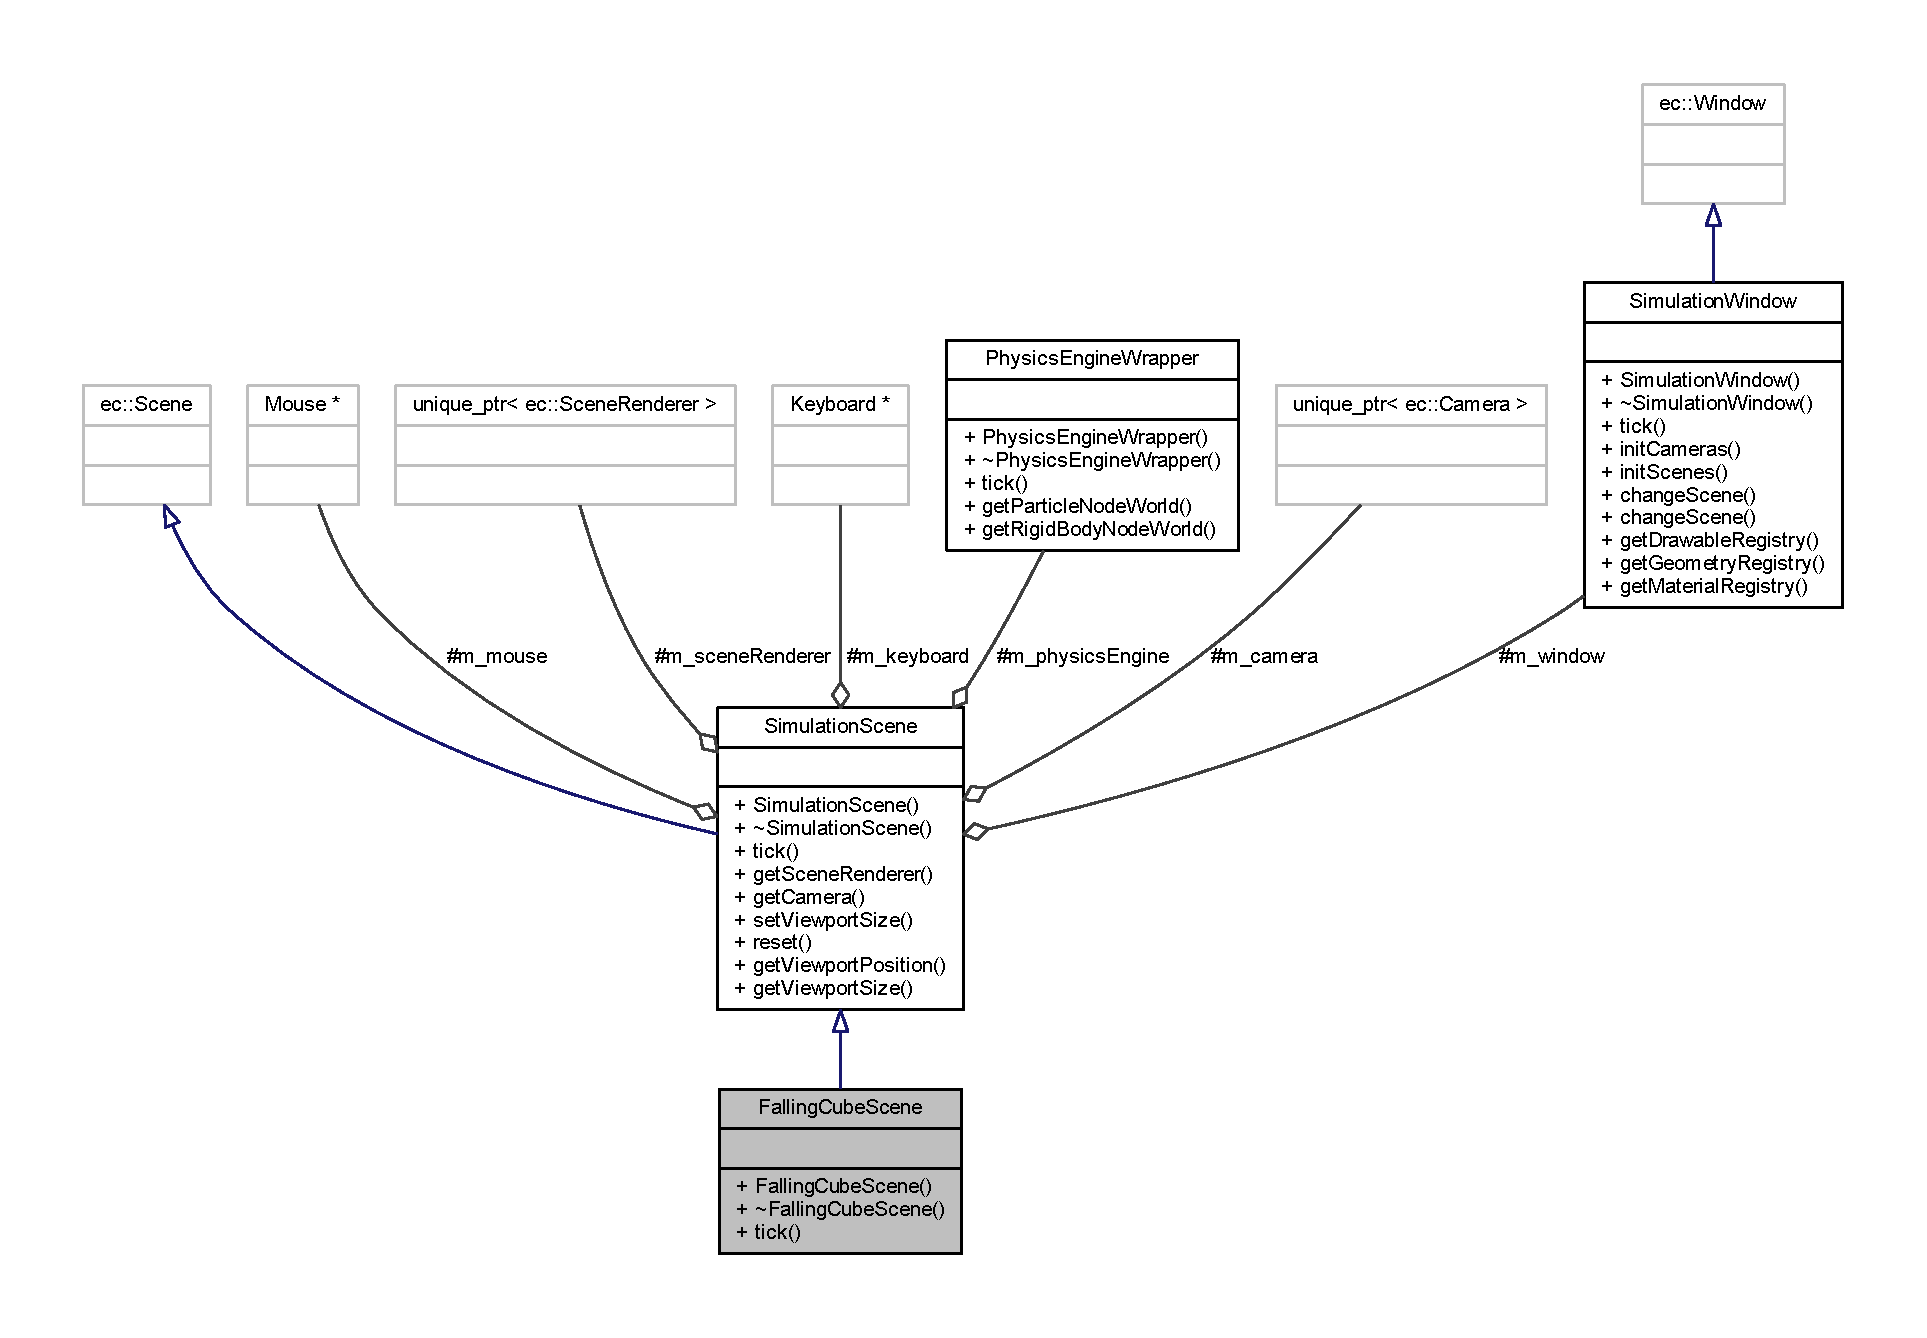
\includegraphics[width=350pt]{class_falling_cube_scene__coll__graph}
\end{center}
\end{figure}
\subsection*{Public Member Functions}
\begin{DoxyCompactItemize}
\item 
\mbox{\hyperlink{class_falling_cube_scene_ab65845f492b9ba6923ca300a426d94c6}{Falling\+Cube\+Scene}} (const std\+::string \&name, \mbox{\hyperlink{class_simulation_window}{Simulation\+Window}} $\ast$window)
\item 
\mbox{\hyperlink{class_falling_cube_scene_a36bf17afa0db6cbf678fa2b1741c2e67}{$\sim$\+Falling\+Cube\+Scene}} ()
\item 
void \mbox{\hyperlink{class_falling_cube_scene_a4d077fc6767b5f5017a35d0433929c27}{tick}} (float time\+Delta) override
\end{DoxyCompactItemize}
\subsection*{Additional Inherited Members}


\subsection{Constructor \& Destructor Documentation}
\mbox{\Hypertarget{class_falling_cube_scene_ab65845f492b9ba6923ca300a426d94c6}\label{class_falling_cube_scene_ab65845f492b9ba6923ca300a426d94c6}} 
\index{Falling\+Cube\+Scene@{Falling\+Cube\+Scene}!Falling\+Cube\+Scene@{Falling\+Cube\+Scene}}
\index{Falling\+Cube\+Scene@{Falling\+Cube\+Scene}!Falling\+Cube\+Scene@{Falling\+Cube\+Scene}}
\subsubsection{\texorpdfstring{Falling\+Cube\+Scene()}{FallingCubeScene()}}
{\footnotesize\ttfamily Falling\+Cube\+Scene\+::\+Falling\+Cube\+Scene (\begin{DoxyParamCaption}\item[{const std\+::string \&}]{name,  }\item[{\mbox{\hyperlink{class_simulation_window}{Simulation\+Window}} $\ast$}]{window }\end{DoxyParamCaption})\hspace{0.3cm}{\ttfamily [explicit]}}

\mbox{\Hypertarget{class_falling_cube_scene_a36bf17afa0db6cbf678fa2b1741c2e67}\label{class_falling_cube_scene_a36bf17afa0db6cbf678fa2b1741c2e67}} 
\index{Falling\+Cube\+Scene@{Falling\+Cube\+Scene}!````~Falling\+Cube\+Scene@{$\sim$\+Falling\+Cube\+Scene}}
\index{````~Falling\+Cube\+Scene@{$\sim$\+Falling\+Cube\+Scene}!Falling\+Cube\+Scene@{Falling\+Cube\+Scene}}
\subsubsection{\texorpdfstring{$\sim$\+Falling\+Cube\+Scene()}{~FallingCubeScene()}}
{\footnotesize\ttfamily Falling\+Cube\+Scene\+::$\sim$\+Falling\+Cube\+Scene (\begin{DoxyParamCaption}{ }\end{DoxyParamCaption})\hspace{0.3cm}{\ttfamily [default]}}



\subsection{Member Function Documentation}
\mbox{\Hypertarget{class_falling_cube_scene_a4d077fc6767b5f5017a35d0433929c27}\label{class_falling_cube_scene_a4d077fc6767b5f5017a35d0433929c27}} 
\index{Falling\+Cube\+Scene@{Falling\+Cube\+Scene}!tick@{tick}}
\index{tick@{tick}!Falling\+Cube\+Scene@{Falling\+Cube\+Scene}}
\subsubsection{\texorpdfstring{tick()}{tick()}}
{\footnotesize\ttfamily void Falling\+Cube\+Scene\+::tick (\begin{DoxyParamCaption}\item[{float}]{time\+Delta }\end{DoxyParamCaption})\hspace{0.3cm}{\ttfamily [override]}}



The documentation for this class was generated from the following files\+:\begin{DoxyCompactItemize}
\item 
D\+:/\+Library/\+Documents/\+Job/\+Forschungsmaster/\+Projekte/\+Simulation\+Visualization/\+Sim/\+Sim/src/\+Examples/\mbox{\hyperlink{_falling_cube_scene_8h}{Falling\+Cube\+Scene.\+h}}\item 
D\+:/\+Library/\+Documents/\+Job/\+Forschungsmaster/\+Projekte/\+Simulation\+Visualization/\+Sim/\+Sim/src/\+Examples/\mbox{\hyperlink{_falling_cube_scene_8cpp}{Falling\+Cube\+Scene.\+cpp}}\end{DoxyCompactItemize}

\hypertarget{class_particle_node}{}\section{Particle\+Node Class Reference}
\label{class_particle_node}\index{Particle\+Node@{Particle\+Node}}


{\ttfamily \#include $<$Particle\+Node.\+h$>$}



Collaboration diagram for Particle\+Node\+:\nopagebreak
\begin{figure}[H]
\begin{center}
\leavevmode
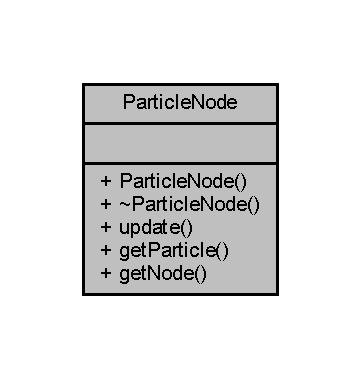
\includegraphics[width=173pt]{class_particle_node__coll__graph}
\end{center}
\end{figure}
\subsection*{Public Member Functions}
\begin{DoxyCompactItemize}
\item 
\mbox{\hyperlink{class_particle_node_a39d9346a90936874b5093445aedca01c}{Particle\+Node}} (r3\+::\+Particle $\ast$particle, ec\+::\+Node $\ast$node)
\item 
\mbox{\hyperlink{class_particle_node_a7ecd9860e75bd4ec3842cc0d0a09cf8b}{$\sim$\+Particle\+Node}} ()
\item 
void \mbox{\hyperlink{class_particle_node_a5324b80595caa65c3e6dbef47ecce09b}{update}} () const
\begin{DoxyCompactList}\small\item\em Update the scene graph node with the associated particle node. \end{DoxyCompactList}\item 
r3\+::\+Particle $\ast$ \mbox{\hyperlink{class_particle_node_a4aaf29e469127cd57a8918f11aacadfb}{get\+Particle}} () const
\begin{DoxyCompactList}\small\item\em Get the current particle. \end{DoxyCompactList}\item 
ec\+::\+Node $\ast$ \mbox{\hyperlink{class_particle_node_add76b91ffda0c229d0d4f1876e671894}{get\+Node}} () const
\end{DoxyCompactItemize}


\subsection{Constructor \& Destructor Documentation}
\mbox{\Hypertarget{class_particle_node_a39d9346a90936874b5093445aedca01c}\label{class_particle_node_a39d9346a90936874b5093445aedca01c}} 
\index{Particle\+Node@{Particle\+Node}!Particle\+Node@{Particle\+Node}}
\index{Particle\+Node@{Particle\+Node}!Particle\+Node@{Particle\+Node}}
\subsubsection{\texorpdfstring{Particle\+Node()}{ParticleNode()}}
{\footnotesize\ttfamily Particle\+Node\+::\+Particle\+Node (\begin{DoxyParamCaption}\item[{r3\+::\+Particle $\ast$}]{particle,  }\item[{ec\+::\+Node $\ast$}]{node }\end{DoxyParamCaption})\hspace{0.3cm}{\ttfamily [explicit]}}

\mbox{\Hypertarget{class_particle_node_a7ecd9860e75bd4ec3842cc0d0a09cf8b}\label{class_particle_node_a7ecd9860e75bd4ec3842cc0d0a09cf8b}} 
\index{Particle\+Node@{Particle\+Node}!````~Particle\+Node@{$\sim$\+Particle\+Node}}
\index{````~Particle\+Node@{$\sim$\+Particle\+Node}!Particle\+Node@{Particle\+Node}}
\subsubsection{\texorpdfstring{$\sim$\+Particle\+Node()}{~ParticleNode()}}
{\footnotesize\ttfamily Particle\+Node\+::$\sim$\+Particle\+Node (\begin{DoxyParamCaption}{ }\end{DoxyParamCaption})\hspace{0.3cm}{\ttfamily [default]}}



\subsection{Member Function Documentation}
\mbox{\Hypertarget{class_particle_node_add76b91ffda0c229d0d4f1876e671894}\label{class_particle_node_add76b91ffda0c229d0d4f1876e671894}} 
\index{Particle\+Node@{Particle\+Node}!get\+Node@{get\+Node}}
\index{get\+Node@{get\+Node}!Particle\+Node@{Particle\+Node}}
\subsubsection{\texorpdfstring{get\+Node()}{getNode()}}
{\footnotesize\ttfamily ec\+::\+Node $\ast$ Particle\+Node\+::get\+Node (\begin{DoxyParamCaption}{ }\end{DoxyParamCaption}) const}

the current node. \mbox{\Hypertarget{class_particle_node_a4aaf29e469127cd57a8918f11aacadfb}\label{class_particle_node_a4aaf29e469127cd57a8918f11aacadfb}} 
\index{Particle\+Node@{Particle\+Node}!get\+Particle@{get\+Particle}}
\index{get\+Particle@{get\+Particle}!Particle\+Node@{Particle\+Node}}
\subsubsection{\texorpdfstring{get\+Particle()}{getParticle()}}
{\footnotesize\ttfamily r3\+::\+Particle $\ast$ Particle\+Node\+::get\+Particle (\begin{DoxyParamCaption}{ }\end{DoxyParamCaption}) const}



Get the current particle. 

\mbox{\Hypertarget{class_particle_node_a5324b80595caa65c3e6dbef47ecce09b}\label{class_particle_node_a5324b80595caa65c3e6dbef47ecce09b}} 
\index{Particle\+Node@{Particle\+Node}!update@{update}}
\index{update@{update}!Particle\+Node@{Particle\+Node}}
\subsubsection{\texorpdfstring{update()}{update()}}
{\footnotesize\ttfamily void Particle\+Node\+::update (\begin{DoxyParamCaption}{ }\end{DoxyParamCaption}) const}



Update the scene graph node with the associated particle node. 



The documentation for this class was generated from the following files\+:\begin{DoxyCompactItemize}
\item 
D\+:/\+Library/\+Documents/\+Job/\+Forschungsmaster/\+Projekte/\+Simulation\+Visualization/\+Sim/\+Sim/src/\+Physic\+Interfaces/\mbox{\hyperlink{_particle_node_8h}{Particle\+Node.\+h}}\item 
D\+:/\+Library/\+Documents/\+Job/\+Forschungsmaster/\+Projekte/\+Simulation\+Visualization/\+Sim/\+Sim/src/\+Physic\+Interfaces/\mbox{\hyperlink{_particle_node_8cpp}{Particle\+Node.\+cpp}}\end{DoxyCompactItemize}

\hypertarget{class_particle_node_world}{}\section{Particle\+Node\+World Class Reference}
\label{class_particle_node_world}\index{Particle\+Node\+World@{Particle\+Node\+World}}


{\ttfamily \#include $<$Particle\+Node\+World.\+h$>$}



Collaboration diagram for Particle\+Node\+World\+:\nopagebreak
\begin{figure}[H]
\begin{center}
\leavevmode
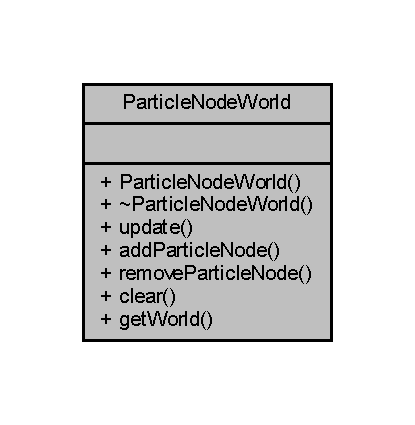
\includegraphics[width=199pt]{class_particle_node_world__coll__graph}
\end{center}
\end{figure}
\subsection*{Public Types}
\begin{DoxyCompactItemize}
\item 
using \mbox{\hyperlink{class_particle_node_world_a7d4a427af20c82cbcba2670899392f33}{Particle\+World\+\_\+\+Ptr}} = std\+::unique\+\_\+ptr$<$ r3\+::\+Particle\+World $>$
\end{DoxyCompactItemize}
\subsection*{Public Member Functions}
\begin{DoxyCompactItemize}
\item 
\mbox{\hyperlink{class_particle_node_world_a54a76a29bfc91fa573d654ba6f582568}{Particle\+Node\+World}} ()
\item 
\mbox{\hyperlink{class_particle_node_world_a7f8e2e6e6f7290c0dc62e1e5ed68ff03}{$\sim$\+Particle\+Node\+World}} ()
\item 
void \mbox{\hyperlink{class_particle_node_world_ad4ec6dd216a026ea9199a3c4b18e380b}{update}} ()
\begin{DoxyCompactList}\small\item\em Update all particle nodes. \end{DoxyCompactList}\item 
void \mbox{\hyperlink{class_particle_node_world_a384ebb3eab353b6508a4eae8d2c8ec95}{add\+Particle\+Node}} (\mbox{\hyperlink{class_particle_node}{Particle\+Node}} $\ast$node)
\begin{DoxyCompactList}\small\item\em Register a new particle node. \end{DoxyCompactList}\item 
bool \mbox{\hyperlink{class_particle_node_world_ae63b0fc7c346b724ae73a050c181d16c}{remove\+Particle\+Node}} (\mbox{\hyperlink{class_particle_node}{Particle\+Node}} $\ast$node)
\begin{DoxyCompactList}\small\item\em Unregister an already registered particle node. \end{DoxyCompactList}\item 
void \mbox{\hyperlink{class_particle_node_world_a19654bc33ccf9caa6265254e13768aa3}{clear}} ()
\begin{DoxyCompactList}\small\item\em Unregister all currently registered particle nodes. \end{DoxyCompactList}\item 
r3\+::\+Particle\+World $\ast$ \mbox{\hyperlink{class_particle_node_world_a116327867d29eedea0781ea604b499ee}{get\+World}} () const
\begin{DoxyCompactList}\small\item\em Get the particle world. \end{DoxyCompactList}\end{DoxyCompactItemize}


\subsection{Member Typedef Documentation}
\mbox{\Hypertarget{class_particle_node_world_a7d4a427af20c82cbcba2670899392f33}\label{class_particle_node_world_a7d4a427af20c82cbcba2670899392f33}} 
\index{Particle\+Node\+World@{Particle\+Node\+World}!Particle\+World\+\_\+\+Ptr@{Particle\+World\+\_\+\+Ptr}}
\index{Particle\+World\+\_\+\+Ptr@{Particle\+World\+\_\+\+Ptr}!Particle\+Node\+World@{Particle\+Node\+World}}
\subsubsection{\texorpdfstring{Particle\+World\+\_\+\+Ptr}{ParticleWorld\_Ptr}}
{\footnotesize\ttfamily using \mbox{\hyperlink{class_particle_node_world_a7d4a427af20c82cbcba2670899392f33}{Particle\+Node\+World\+::\+Particle\+World\+\_\+\+Ptr}} =  std\+::unique\+\_\+ptr$<$r3\+::\+Particle\+World$>$}



\subsection{Constructor \& Destructor Documentation}
\mbox{\Hypertarget{class_particle_node_world_a54a76a29bfc91fa573d654ba6f582568}\label{class_particle_node_world_a54a76a29bfc91fa573d654ba6f582568}} 
\index{Particle\+Node\+World@{Particle\+Node\+World}!Particle\+Node\+World@{Particle\+Node\+World}}
\index{Particle\+Node\+World@{Particle\+Node\+World}!Particle\+Node\+World@{Particle\+Node\+World}}
\subsubsection{\texorpdfstring{Particle\+Node\+World()}{ParticleNodeWorld()}}
{\footnotesize\ttfamily Particle\+Node\+World\+::\+Particle\+Node\+World (\begin{DoxyParamCaption}{ }\end{DoxyParamCaption})\hspace{0.3cm}{\ttfamily [explicit]}}

\mbox{\Hypertarget{class_particle_node_world_a7f8e2e6e6f7290c0dc62e1e5ed68ff03}\label{class_particle_node_world_a7f8e2e6e6f7290c0dc62e1e5ed68ff03}} 
\index{Particle\+Node\+World@{Particle\+Node\+World}!````~Particle\+Node\+World@{$\sim$\+Particle\+Node\+World}}
\index{````~Particle\+Node\+World@{$\sim$\+Particle\+Node\+World}!Particle\+Node\+World@{Particle\+Node\+World}}
\subsubsection{\texorpdfstring{$\sim$\+Particle\+Node\+World()}{~ParticleNodeWorld()}}
{\footnotesize\ttfamily Particle\+Node\+World\+::$\sim$\+Particle\+Node\+World (\begin{DoxyParamCaption}{ }\end{DoxyParamCaption})\hspace{0.3cm}{\ttfamily [default]}}



\subsection{Member Function Documentation}
\mbox{\Hypertarget{class_particle_node_world_a384ebb3eab353b6508a4eae8d2c8ec95}\label{class_particle_node_world_a384ebb3eab353b6508a4eae8d2c8ec95}} 
\index{Particle\+Node\+World@{Particle\+Node\+World}!add\+Particle\+Node@{add\+Particle\+Node}}
\index{add\+Particle\+Node@{add\+Particle\+Node}!Particle\+Node\+World@{Particle\+Node\+World}}
\subsubsection{\texorpdfstring{add\+Particle\+Node()}{addParticleNode()}}
{\footnotesize\ttfamily void Particle\+Node\+World\+::add\+Particle\+Node (\begin{DoxyParamCaption}\item[{\mbox{\hyperlink{class_particle_node}{Particle\+Node}} $\ast$}]{node }\end{DoxyParamCaption})}



Register a new particle node. 

\mbox{\Hypertarget{class_particle_node_world_a19654bc33ccf9caa6265254e13768aa3}\label{class_particle_node_world_a19654bc33ccf9caa6265254e13768aa3}} 
\index{Particle\+Node\+World@{Particle\+Node\+World}!clear@{clear}}
\index{clear@{clear}!Particle\+Node\+World@{Particle\+Node\+World}}
\subsubsection{\texorpdfstring{clear()}{clear()}}
{\footnotesize\ttfamily void Particle\+Node\+World\+::clear (\begin{DoxyParamCaption}{ }\end{DoxyParamCaption})}



Unregister all currently registered particle nodes. 

\mbox{\Hypertarget{class_particle_node_world_a116327867d29eedea0781ea604b499ee}\label{class_particle_node_world_a116327867d29eedea0781ea604b499ee}} 
\index{Particle\+Node\+World@{Particle\+Node\+World}!get\+World@{get\+World}}
\index{get\+World@{get\+World}!Particle\+Node\+World@{Particle\+Node\+World}}
\subsubsection{\texorpdfstring{get\+World()}{getWorld()}}
{\footnotesize\ttfamily r3\+::\+Particle\+World $\ast$ Particle\+Node\+World\+::get\+World (\begin{DoxyParamCaption}{ }\end{DoxyParamCaption}) const}



Get the particle world. 

\mbox{\Hypertarget{class_particle_node_world_ae63b0fc7c346b724ae73a050c181d16c}\label{class_particle_node_world_ae63b0fc7c346b724ae73a050c181d16c}} 
\index{Particle\+Node\+World@{Particle\+Node\+World}!remove\+Particle\+Node@{remove\+Particle\+Node}}
\index{remove\+Particle\+Node@{remove\+Particle\+Node}!Particle\+Node\+World@{Particle\+Node\+World}}
\subsubsection{\texorpdfstring{remove\+Particle\+Node()}{removeParticleNode()}}
{\footnotesize\ttfamily bool Particle\+Node\+World\+::remove\+Particle\+Node (\begin{DoxyParamCaption}\item[{\mbox{\hyperlink{class_particle_node}{Particle\+Node}} $\ast$}]{node }\end{DoxyParamCaption})}



Unregister an already registered particle node. 

\mbox{\Hypertarget{class_particle_node_world_ad4ec6dd216a026ea9199a3c4b18e380b}\label{class_particle_node_world_ad4ec6dd216a026ea9199a3c4b18e380b}} 
\index{Particle\+Node\+World@{Particle\+Node\+World}!update@{update}}
\index{update@{update}!Particle\+Node\+World@{Particle\+Node\+World}}
\subsubsection{\texorpdfstring{update()}{update()}}
{\footnotesize\ttfamily void Particle\+Node\+World\+::update (\begin{DoxyParamCaption}{ }\end{DoxyParamCaption})}



Update all particle nodes. 



The documentation for this class was generated from the following files\+:\begin{DoxyCompactItemize}
\item 
D\+:/\+Library/\+Documents/\+Job/\+Forschungsmaster/\+Projekte/\+Simulation\+Visualization/\+Sim/\+Sim/src/\+Physic\+Interfaces/\mbox{\hyperlink{_particle_node_world_8h}{Particle\+Node\+World.\+h}}\item 
D\+:/\+Library/\+Documents/\+Job/\+Forschungsmaster/\+Projekte/\+Simulation\+Visualization/\+Sim/\+Sim/src/\+Physic\+Interfaces/\mbox{\hyperlink{_particle_node_world_8cpp}{Particle\+Node\+World.\+cpp}}\end{DoxyCompactItemize}

\hypertarget{class_physics_engine_wrapper}{}\section{Physics\+Engine\+Wrapper Class Reference}
\label{class_physics_engine_wrapper}\index{Physics\+Engine\+Wrapper@{Physics\+Engine\+Wrapper}}


{\ttfamily \#include $<$Physics\+Engine\+Wrapper.\+h$>$}



Collaboration diagram for Physics\+Engine\+Wrapper\+:\nopagebreak
\begin{figure}[H]
\begin{center}
\leavevmode
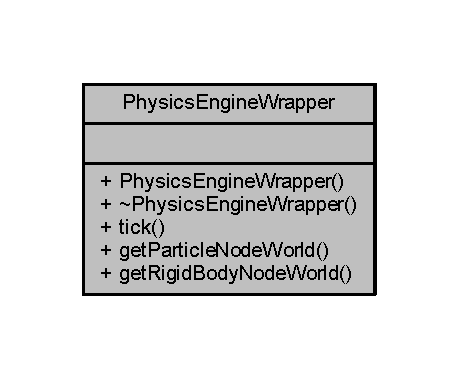
\includegraphics[width=220pt]{class_physics_engine_wrapper__coll__graph}
\end{center}
\end{figure}
\subsection*{Public Types}
\begin{DoxyCompactItemize}
\item 
using \mbox{\hyperlink{class_physics_engine_wrapper_a842bf2a6668082cbc4568e0212d16cc9}{Particle\+Node\+World\+\_\+\+Ptr}} = std\+::unique\+\_\+ptr$<$ \mbox{\hyperlink{class_particle_node_world}{Particle\+Node\+World}} $>$
\item 
using \mbox{\hyperlink{class_physics_engine_wrapper_a3c72d58c14dbb32642177a6a7aa73368}{Rigid\+Body\+Node\+World\+\_\+\+Ptr}} = std\+::unique\+\_\+ptr$<$ \mbox{\hyperlink{class_rigid_body_node_world}{Rigid\+Body\+Node\+World}} $>$
\end{DoxyCompactItemize}
\subsection*{Public Member Functions}
\begin{DoxyCompactItemize}
\item 
\mbox{\hyperlink{class_physics_engine_wrapper_a9927ccae5bfa6fff5a329bcd55fdb006}{Physics\+Engine\+Wrapper}} ()
\item 
\mbox{\hyperlink{class_physics_engine_wrapper_aa918612e647ac8e0d5510d991752096e}{$\sim$\+Physics\+Engine\+Wrapper}} ()
\item 
void \mbox{\hyperlink{class_physics_engine_wrapper_ab373f860362e7c74dfa0eabfffe10bec}{tick}} (float time\+Delta)
\item 
\mbox{\hyperlink{class_particle_node_world}{Particle\+Node\+World}} $\ast$ \mbox{\hyperlink{class_physics_engine_wrapper_a616efbb6a5a787618e0d07eef552e876}{get\+Particle\+Node\+World}} () const
\item 
\mbox{\hyperlink{class_rigid_body_node_world}{Rigid\+Body\+Node\+World}} $\ast$ \mbox{\hyperlink{class_physics_engine_wrapper_af5d784792df1ea0186bcf21fd0c7d115}{get\+Rigid\+Body\+Node\+World}} () const
\end{DoxyCompactItemize}


\subsection{Member Typedef Documentation}
\mbox{\Hypertarget{class_physics_engine_wrapper_a842bf2a6668082cbc4568e0212d16cc9}\label{class_physics_engine_wrapper_a842bf2a6668082cbc4568e0212d16cc9}} 
\index{Physics\+Engine\+Wrapper@{Physics\+Engine\+Wrapper}!Particle\+Node\+World\+\_\+\+Ptr@{Particle\+Node\+World\+\_\+\+Ptr}}
\index{Particle\+Node\+World\+\_\+\+Ptr@{Particle\+Node\+World\+\_\+\+Ptr}!Physics\+Engine\+Wrapper@{Physics\+Engine\+Wrapper}}
\subsubsection{\texorpdfstring{Particle\+Node\+World\+\_\+\+Ptr}{ParticleNodeWorld\_Ptr}}
{\footnotesize\ttfamily using \mbox{\hyperlink{class_physics_engine_wrapper_a842bf2a6668082cbc4568e0212d16cc9}{Physics\+Engine\+Wrapper\+::\+Particle\+Node\+World\+\_\+\+Ptr}} =  std\+::unique\+\_\+ptr$<$\mbox{\hyperlink{class_particle_node_world}{Particle\+Node\+World}}$>$}

\mbox{\Hypertarget{class_physics_engine_wrapper_a3c72d58c14dbb32642177a6a7aa73368}\label{class_physics_engine_wrapper_a3c72d58c14dbb32642177a6a7aa73368}} 
\index{Physics\+Engine\+Wrapper@{Physics\+Engine\+Wrapper}!Rigid\+Body\+Node\+World\+\_\+\+Ptr@{Rigid\+Body\+Node\+World\+\_\+\+Ptr}}
\index{Rigid\+Body\+Node\+World\+\_\+\+Ptr@{Rigid\+Body\+Node\+World\+\_\+\+Ptr}!Physics\+Engine\+Wrapper@{Physics\+Engine\+Wrapper}}
\subsubsection{\texorpdfstring{Rigid\+Body\+Node\+World\+\_\+\+Ptr}{RigidBodyNodeWorld\_Ptr}}
{\footnotesize\ttfamily using \mbox{\hyperlink{class_physics_engine_wrapper_a3c72d58c14dbb32642177a6a7aa73368}{Physics\+Engine\+Wrapper\+::\+Rigid\+Body\+Node\+World\+\_\+\+Ptr}} =  std\+::unique\+\_\+ptr$<$\mbox{\hyperlink{class_rigid_body_node_world}{Rigid\+Body\+Node\+World}}$>$}



\subsection{Constructor \& Destructor Documentation}
\mbox{\Hypertarget{class_physics_engine_wrapper_a9927ccae5bfa6fff5a329bcd55fdb006}\label{class_physics_engine_wrapper_a9927ccae5bfa6fff5a329bcd55fdb006}} 
\index{Physics\+Engine\+Wrapper@{Physics\+Engine\+Wrapper}!Physics\+Engine\+Wrapper@{Physics\+Engine\+Wrapper}}
\index{Physics\+Engine\+Wrapper@{Physics\+Engine\+Wrapper}!Physics\+Engine\+Wrapper@{Physics\+Engine\+Wrapper}}
\subsubsection{\texorpdfstring{Physics\+Engine\+Wrapper()}{PhysicsEngineWrapper()}}
{\footnotesize\ttfamily Physics\+Engine\+Wrapper\+::\+Physics\+Engine\+Wrapper (\begin{DoxyParamCaption}{ }\end{DoxyParamCaption})\hspace{0.3cm}{\ttfamily [explicit]}}

\mbox{\Hypertarget{class_physics_engine_wrapper_aa918612e647ac8e0d5510d991752096e}\label{class_physics_engine_wrapper_aa918612e647ac8e0d5510d991752096e}} 
\index{Physics\+Engine\+Wrapper@{Physics\+Engine\+Wrapper}!````~Physics\+Engine\+Wrapper@{$\sim$\+Physics\+Engine\+Wrapper}}
\index{````~Physics\+Engine\+Wrapper@{$\sim$\+Physics\+Engine\+Wrapper}!Physics\+Engine\+Wrapper@{Physics\+Engine\+Wrapper}}
\subsubsection{\texorpdfstring{$\sim$\+Physics\+Engine\+Wrapper()}{~PhysicsEngineWrapper()}}
{\footnotesize\ttfamily Physics\+Engine\+Wrapper\+::$\sim$\+Physics\+Engine\+Wrapper (\begin{DoxyParamCaption}{ }\end{DoxyParamCaption})\hspace{0.3cm}{\ttfamily [default]}}



\subsection{Member Function Documentation}
\mbox{\Hypertarget{class_physics_engine_wrapper_a616efbb6a5a787618e0d07eef552e876}\label{class_physics_engine_wrapper_a616efbb6a5a787618e0d07eef552e876}} 
\index{Physics\+Engine\+Wrapper@{Physics\+Engine\+Wrapper}!get\+Particle\+Node\+World@{get\+Particle\+Node\+World}}
\index{get\+Particle\+Node\+World@{get\+Particle\+Node\+World}!Physics\+Engine\+Wrapper@{Physics\+Engine\+Wrapper}}
\subsubsection{\texorpdfstring{get\+Particle\+Node\+World()}{getParticleNodeWorld()}}
{\footnotesize\ttfamily \mbox{\hyperlink{class_particle_node_world}{Particle\+Node\+World}} $\ast$ Physics\+Engine\+Wrapper\+::get\+Particle\+Node\+World (\begin{DoxyParamCaption}{ }\end{DoxyParamCaption}) const}

\mbox{\Hypertarget{class_physics_engine_wrapper_af5d784792df1ea0186bcf21fd0c7d115}\label{class_physics_engine_wrapper_af5d784792df1ea0186bcf21fd0c7d115}} 
\index{Physics\+Engine\+Wrapper@{Physics\+Engine\+Wrapper}!get\+Rigid\+Body\+Node\+World@{get\+Rigid\+Body\+Node\+World}}
\index{get\+Rigid\+Body\+Node\+World@{get\+Rigid\+Body\+Node\+World}!Physics\+Engine\+Wrapper@{Physics\+Engine\+Wrapper}}
\subsubsection{\texorpdfstring{get\+Rigid\+Body\+Node\+World()}{getRigidBodyNodeWorld()}}
{\footnotesize\ttfamily \mbox{\hyperlink{class_rigid_body_node_world}{Rigid\+Body\+Node\+World}} $\ast$ Physics\+Engine\+Wrapper\+::get\+Rigid\+Body\+Node\+World (\begin{DoxyParamCaption}{ }\end{DoxyParamCaption}) const}

\mbox{\Hypertarget{class_physics_engine_wrapper_ab373f860362e7c74dfa0eabfffe10bec}\label{class_physics_engine_wrapper_ab373f860362e7c74dfa0eabfffe10bec}} 
\index{Physics\+Engine\+Wrapper@{Physics\+Engine\+Wrapper}!tick@{tick}}
\index{tick@{tick}!Physics\+Engine\+Wrapper@{Physics\+Engine\+Wrapper}}
\subsubsection{\texorpdfstring{tick()}{tick()}}
{\footnotesize\ttfamily void Physics\+Engine\+Wrapper\+::tick (\begin{DoxyParamCaption}\item[{float}]{time\+Delta }\end{DoxyParamCaption})}



The documentation for this class was generated from the following files\+:\begin{DoxyCompactItemize}
\item 
D\+:/\+Library/\+Documents/\+Job/\+Forschungsmaster/\+Projekte/\+Simulation\+Visualization/\+Sim/\+Sim/src/\+Physic\+Interfaces/\mbox{\hyperlink{_physics_engine_wrapper_8h}{Physics\+Engine\+Wrapper.\+h}}\item 
D\+:/\+Library/\+Documents/\+Job/\+Forschungsmaster/\+Projekte/\+Simulation\+Visualization/\+Sim/\+Sim/src/\+Physic\+Interfaces/\mbox{\hyperlink{_physics_engine_wrapper_8cpp}{Physics\+Engine\+Wrapper.\+cpp}}\end{DoxyCompactItemize}

\hypertarget{class_rigid_body_node}{}\section{Rigid\+Body\+Node Class Reference}
\label{class_rigid_body_node}\index{Rigid\+Body\+Node@{Rigid\+Body\+Node}}


{\ttfamily \#include $<$Rigid\+Body\+Node.\+h$>$}



Collaboration diagram for Rigid\+Body\+Node\+:\nopagebreak
\begin{figure}[H]
\begin{center}
\leavevmode
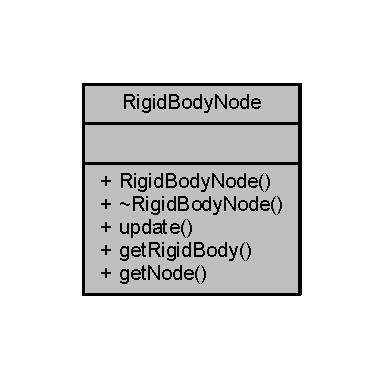
\includegraphics[width=184pt]{class_rigid_body_node__coll__graph}
\end{center}
\end{figure}
\subsection*{Public Member Functions}
\begin{DoxyCompactItemize}
\item 
\mbox{\hyperlink{class_rigid_body_node_a8ce6244b5ddff6ffcae6273e2613ec7c}{Rigid\+Body\+Node}} (r3\+::\+Rigid\+Body $\ast$rigid\+Body, ec\+::\+Node $\ast$node)
\item 
\mbox{\hyperlink{class_rigid_body_node_a9fab17e299f7e471c726d644cb65aedf}{$\sim$\+Rigid\+Body\+Node}} ()
\item 
void \mbox{\hyperlink{class_rigid_body_node_aa40aff305449fa4b1d8b1c665548f862}{update}} () const
\begin{DoxyCompactList}\small\item\em Update the scene graph node with the associated rigid body node. \end{DoxyCompactList}\item 
r3\+::\+Rigid\+Body $\ast$ \mbox{\hyperlink{class_rigid_body_node_ab1a0b587bed1ff3298da3b382ada784f}{get\+Rigid\+Body}} () const
\begin{DoxyCompactList}\small\item\em Get the current rigid body. \end{DoxyCompactList}\item 
ec\+::\+Node $\ast$ \mbox{\hyperlink{class_rigid_body_node_a1004482a1aa31b8bd7df515815b0fc59}{get\+Node}} () const
\begin{DoxyCompactList}\small\item\em Get the current node. \end{DoxyCompactList}\end{DoxyCompactItemize}


\subsection{Constructor \& Destructor Documentation}
\mbox{\Hypertarget{class_rigid_body_node_a8ce6244b5ddff6ffcae6273e2613ec7c}\label{class_rigid_body_node_a8ce6244b5ddff6ffcae6273e2613ec7c}} 
\index{Rigid\+Body\+Node@{Rigid\+Body\+Node}!Rigid\+Body\+Node@{Rigid\+Body\+Node}}
\index{Rigid\+Body\+Node@{Rigid\+Body\+Node}!Rigid\+Body\+Node@{Rigid\+Body\+Node}}
\subsubsection{\texorpdfstring{Rigid\+Body\+Node()}{RigidBodyNode()}}
{\footnotesize\ttfamily Rigid\+Body\+Node\+::\+Rigid\+Body\+Node (\begin{DoxyParamCaption}\item[{r3\+::\+Rigid\+Body $\ast$}]{rigid\+Body,  }\item[{ec\+::\+Node $\ast$}]{node }\end{DoxyParamCaption})}

\mbox{\Hypertarget{class_rigid_body_node_a9fab17e299f7e471c726d644cb65aedf}\label{class_rigid_body_node_a9fab17e299f7e471c726d644cb65aedf}} 
\index{Rigid\+Body\+Node@{Rigid\+Body\+Node}!````~Rigid\+Body\+Node@{$\sim$\+Rigid\+Body\+Node}}
\index{````~Rigid\+Body\+Node@{$\sim$\+Rigid\+Body\+Node}!Rigid\+Body\+Node@{Rigid\+Body\+Node}}
\subsubsection{\texorpdfstring{$\sim$\+Rigid\+Body\+Node()}{~RigidBodyNode()}}
{\footnotesize\ttfamily Rigid\+Body\+Node\+::$\sim$\+Rigid\+Body\+Node (\begin{DoxyParamCaption}{ }\end{DoxyParamCaption})\hspace{0.3cm}{\ttfamily [default]}}



\subsection{Member Function Documentation}
\mbox{\Hypertarget{class_rigid_body_node_a1004482a1aa31b8bd7df515815b0fc59}\label{class_rigid_body_node_a1004482a1aa31b8bd7df515815b0fc59}} 
\index{Rigid\+Body\+Node@{Rigid\+Body\+Node}!get\+Node@{get\+Node}}
\index{get\+Node@{get\+Node}!Rigid\+Body\+Node@{Rigid\+Body\+Node}}
\subsubsection{\texorpdfstring{get\+Node()}{getNode()}}
{\footnotesize\ttfamily ec\+::\+Node $\ast$ Rigid\+Body\+Node\+::get\+Node (\begin{DoxyParamCaption}{ }\end{DoxyParamCaption}) const}



Get the current node. 

\mbox{\Hypertarget{class_rigid_body_node_ab1a0b587bed1ff3298da3b382ada784f}\label{class_rigid_body_node_ab1a0b587bed1ff3298da3b382ada784f}} 
\index{Rigid\+Body\+Node@{Rigid\+Body\+Node}!get\+Rigid\+Body@{get\+Rigid\+Body}}
\index{get\+Rigid\+Body@{get\+Rigid\+Body}!Rigid\+Body\+Node@{Rigid\+Body\+Node}}
\subsubsection{\texorpdfstring{get\+Rigid\+Body()}{getRigidBody()}}
{\footnotesize\ttfamily r3\+::\+Rigid\+Body $\ast$ Rigid\+Body\+Node\+::get\+Rigid\+Body (\begin{DoxyParamCaption}{ }\end{DoxyParamCaption}) const}



Get the current rigid body. 

\mbox{\Hypertarget{class_rigid_body_node_aa40aff305449fa4b1d8b1c665548f862}\label{class_rigid_body_node_aa40aff305449fa4b1d8b1c665548f862}} 
\index{Rigid\+Body\+Node@{Rigid\+Body\+Node}!update@{update}}
\index{update@{update}!Rigid\+Body\+Node@{Rigid\+Body\+Node}}
\subsubsection{\texorpdfstring{update()}{update()}}
{\footnotesize\ttfamily void Rigid\+Body\+Node\+::update (\begin{DoxyParamCaption}{ }\end{DoxyParamCaption}) const}



Update the scene graph node with the associated rigid body node. 



The documentation for this class was generated from the following files\+:\begin{DoxyCompactItemize}
\item 
D\+:/\+Library/\+Documents/\+Job/\+Forschungsmaster/\+Projekte/\+Simulation\+Visualization/\+Sim/\+Sim/src/\+Physic\+Interfaces/\mbox{\hyperlink{_rigid_body_node_8h}{Rigid\+Body\+Node.\+h}}\item 
D\+:/\+Library/\+Documents/\+Job/\+Forschungsmaster/\+Projekte/\+Simulation\+Visualization/\+Sim/\+Sim/src/\+Physic\+Interfaces/\mbox{\hyperlink{_rigid_body_node_8cpp}{Rigid\+Body\+Node.\+cpp}}\end{DoxyCompactItemize}

\hypertarget{class_rigid_body_node_world}{}\section{Rigid\+Body\+Node\+World Class Reference}
\label{class_rigid_body_node_world}\index{Rigid\+Body\+Node\+World@{Rigid\+Body\+Node\+World}}


{\ttfamily \#include $<$Rigid\+Body\+Node\+World.\+h$>$}



Collaboration diagram for Rigid\+Body\+Node\+World\+:\nopagebreak
\begin{figure}[H]
\begin{center}
\leavevmode
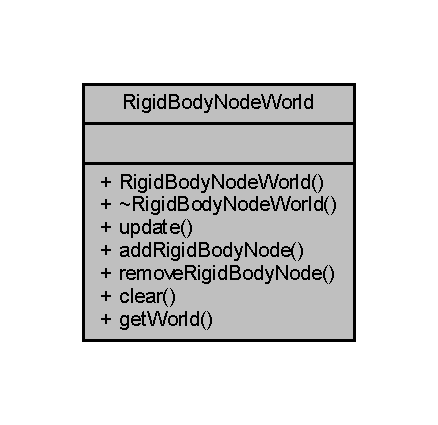
\includegraphics[width=210pt]{class_rigid_body_node_world__coll__graph}
\end{center}
\end{figure}
\subsection*{Public Types}
\begin{DoxyCompactItemize}
\item 
using \mbox{\hyperlink{class_rigid_body_node_world_a34a1badfc25cc91284fb98c9421bd35a}{Rigid\+Body\+World\+\_\+\+Ptr}} = std\+::unique\+\_\+ptr$<$ r3\+::\+Rigid\+Body\+World $>$
\end{DoxyCompactItemize}
\subsection*{Public Member Functions}
\begin{DoxyCompactItemize}
\item 
\mbox{\hyperlink{class_rigid_body_node_world_a44345ab3fc624d3d100974f854468f68}{Rigid\+Body\+Node\+World}} ()
\item 
\mbox{\hyperlink{class_rigid_body_node_world_ac6a0800e44f827f97f3da6c68b53eabd}{$\sim$\+Rigid\+Body\+Node\+World}} ()
\item 
void \mbox{\hyperlink{class_rigid_body_node_world_a3b381c6da9b1374eb12117c6e8d0b57a}{update}} ()
\begin{DoxyCompactList}\small\item\em Update all registered rigid body nodes. \end{DoxyCompactList}\item 
void \mbox{\hyperlink{class_rigid_body_node_world_a1dc9da65de6b73fe78b08523eb7c6d5f}{add\+Rigid\+Body\+Node}} (\mbox{\hyperlink{class_rigid_body_node}{Rigid\+Body\+Node}} $\ast$node)
\begin{DoxyCompactList}\small\item\em Register a new rigid body node. \end{DoxyCompactList}\item 
bool \mbox{\hyperlink{class_rigid_body_node_world_a444034dce9139e77f7714779afb04235}{remove\+Rigid\+Body\+Node}} (\mbox{\hyperlink{class_rigid_body_node}{Rigid\+Body\+Node}} $\ast$node)
\begin{DoxyCompactList}\small\item\em Unregister an already registered rigid body node. \end{DoxyCompactList}\item 
void \mbox{\hyperlink{class_rigid_body_node_world_a3795fdb1b75c0da1286627e2c9b63830}{clear}} ()
\begin{DoxyCompactList}\small\item\em Unregister all currently registered rigid body nodes. \end{DoxyCompactList}\item 
r3\+::\+Rigid\+Body\+World $\ast$ \mbox{\hyperlink{class_rigid_body_node_world_aa1ddbb33d36e112134c54cbb5483df26}{get\+World}} () const
\begin{DoxyCompactList}\small\item\em Get the rigid body world. \end{DoxyCompactList}\end{DoxyCompactItemize}


\subsection{Member Typedef Documentation}
\mbox{\Hypertarget{class_rigid_body_node_world_a34a1badfc25cc91284fb98c9421bd35a}\label{class_rigid_body_node_world_a34a1badfc25cc91284fb98c9421bd35a}} 
\index{Rigid\+Body\+Node\+World@{Rigid\+Body\+Node\+World}!Rigid\+Body\+World\+\_\+\+Ptr@{Rigid\+Body\+World\+\_\+\+Ptr}}
\index{Rigid\+Body\+World\+\_\+\+Ptr@{Rigid\+Body\+World\+\_\+\+Ptr}!Rigid\+Body\+Node\+World@{Rigid\+Body\+Node\+World}}
\subsubsection{\texorpdfstring{Rigid\+Body\+World\+\_\+\+Ptr}{RigidBodyWorld\_Ptr}}
{\footnotesize\ttfamily using \mbox{\hyperlink{class_rigid_body_node_world_a34a1badfc25cc91284fb98c9421bd35a}{Rigid\+Body\+Node\+World\+::\+Rigid\+Body\+World\+\_\+\+Ptr}} =  std\+::unique\+\_\+ptr$<$r3\+::\+Rigid\+Body\+World$>$}



\subsection{Constructor \& Destructor Documentation}
\mbox{\Hypertarget{class_rigid_body_node_world_a44345ab3fc624d3d100974f854468f68}\label{class_rigid_body_node_world_a44345ab3fc624d3d100974f854468f68}} 
\index{Rigid\+Body\+Node\+World@{Rigid\+Body\+Node\+World}!Rigid\+Body\+Node\+World@{Rigid\+Body\+Node\+World}}
\index{Rigid\+Body\+Node\+World@{Rigid\+Body\+Node\+World}!Rigid\+Body\+Node\+World@{Rigid\+Body\+Node\+World}}
\subsubsection{\texorpdfstring{Rigid\+Body\+Node\+World()}{RigidBodyNodeWorld()}}
{\footnotesize\ttfamily Rigid\+Body\+Node\+World\+::\+Rigid\+Body\+Node\+World (\begin{DoxyParamCaption}{ }\end{DoxyParamCaption})\hspace{0.3cm}{\ttfamily [explicit]}}

\mbox{\Hypertarget{class_rigid_body_node_world_ac6a0800e44f827f97f3da6c68b53eabd}\label{class_rigid_body_node_world_ac6a0800e44f827f97f3da6c68b53eabd}} 
\index{Rigid\+Body\+Node\+World@{Rigid\+Body\+Node\+World}!````~Rigid\+Body\+Node\+World@{$\sim$\+Rigid\+Body\+Node\+World}}
\index{````~Rigid\+Body\+Node\+World@{$\sim$\+Rigid\+Body\+Node\+World}!Rigid\+Body\+Node\+World@{Rigid\+Body\+Node\+World}}
\subsubsection{\texorpdfstring{$\sim$\+Rigid\+Body\+Node\+World()}{~RigidBodyNodeWorld()}}
{\footnotesize\ttfamily Rigid\+Body\+Node\+World\+::$\sim$\+Rigid\+Body\+Node\+World (\begin{DoxyParamCaption}{ }\end{DoxyParamCaption})\hspace{0.3cm}{\ttfamily [default]}}



\subsection{Member Function Documentation}
\mbox{\Hypertarget{class_rigid_body_node_world_a1dc9da65de6b73fe78b08523eb7c6d5f}\label{class_rigid_body_node_world_a1dc9da65de6b73fe78b08523eb7c6d5f}} 
\index{Rigid\+Body\+Node\+World@{Rigid\+Body\+Node\+World}!add\+Rigid\+Body\+Node@{add\+Rigid\+Body\+Node}}
\index{add\+Rigid\+Body\+Node@{add\+Rigid\+Body\+Node}!Rigid\+Body\+Node\+World@{Rigid\+Body\+Node\+World}}
\subsubsection{\texorpdfstring{add\+Rigid\+Body\+Node()}{addRigidBodyNode()}}
{\footnotesize\ttfamily void Rigid\+Body\+Node\+World\+::add\+Rigid\+Body\+Node (\begin{DoxyParamCaption}\item[{\mbox{\hyperlink{class_rigid_body_node}{Rigid\+Body\+Node}} $\ast$}]{node }\end{DoxyParamCaption})}



Register a new rigid body node. 

\mbox{\Hypertarget{class_rigid_body_node_world_a3795fdb1b75c0da1286627e2c9b63830}\label{class_rigid_body_node_world_a3795fdb1b75c0da1286627e2c9b63830}} 
\index{Rigid\+Body\+Node\+World@{Rigid\+Body\+Node\+World}!clear@{clear}}
\index{clear@{clear}!Rigid\+Body\+Node\+World@{Rigid\+Body\+Node\+World}}
\subsubsection{\texorpdfstring{clear()}{clear()}}
{\footnotesize\ttfamily void Rigid\+Body\+Node\+World\+::clear (\begin{DoxyParamCaption}{ }\end{DoxyParamCaption})}



Unregister all currently registered rigid body nodes. 

\mbox{\Hypertarget{class_rigid_body_node_world_aa1ddbb33d36e112134c54cbb5483df26}\label{class_rigid_body_node_world_aa1ddbb33d36e112134c54cbb5483df26}} 
\index{Rigid\+Body\+Node\+World@{Rigid\+Body\+Node\+World}!get\+World@{get\+World}}
\index{get\+World@{get\+World}!Rigid\+Body\+Node\+World@{Rigid\+Body\+Node\+World}}
\subsubsection{\texorpdfstring{get\+World()}{getWorld()}}
{\footnotesize\ttfamily r3\+::\+Rigid\+Body\+World $\ast$ Rigid\+Body\+Node\+World\+::get\+World (\begin{DoxyParamCaption}{ }\end{DoxyParamCaption}) const}



Get the rigid body world. 

\mbox{\Hypertarget{class_rigid_body_node_world_a444034dce9139e77f7714779afb04235}\label{class_rigid_body_node_world_a444034dce9139e77f7714779afb04235}} 
\index{Rigid\+Body\+Node\+World@{Rigid\+Body\+Node\+World}!remove\+Rigid\+Body\+Node@{remove\+Rigid\+Body\+Node}}
\index{remove\+Rigid\+Body\+Node@{remove\+Rigid\+Body\+Node}!Rigid\+Body\+Node\+World@{Rigid\+Body\+Node\+World}}
\subsubsection{\texorpdfstring{remove\+Rigid\+Body\+Node()}{removeRigidBodyNode()}}
{\footnotesize\ttfamily bool Rigid\+Body\+Node\+World\+::remove\+Rigid\+Body\+Node (\begin{DoxyParamCaption}\item[{\mbox{\hyperlink{class_rigid_body_node}{Rigid\+Body\+Node}} $\ast$}]{node }\end{DoxyParamCaption})}



Unregister an already registered rigid body node. 

\begin{DoxyReturn}{Returns}
True if the rigid body node was found, false otherwise. 
\end{DoxyReturn}
\mbox{\Hypertarget{class_rigid_body_node_world_a3b381c6da9b1374eb12117c6e8d0b57a}\label{class_rigid_body_node_world_a3b381c6da9b1374eb12117c6e8d0b57a}} 
\index{Rigid\+Body\+Node\+World@{Rigid\+Body\+Node\+World}!update@{update}}
\index{update@{update}!Rigid\+Body\+Node\+World@{Rigid\+Body\+Node\+World}}
\subsubsection{\texorpdfstring{update()}{update()}}
{\footnotesize\ttfamily void Rigid\+Body\+Node\+World\+::update (\begin{DoxyParamCaption}{ }\end{DoxyParamCaption})}



Update all registered rigid body nodes. 



The documentation for this class was generated from the following files\+:\begin{DoxyCompactItemize}
\item 
D\+:/\+Library/\+Documents/\+Job/\+Forschungsmaster/\+Projekte/\+Simulation\+Visualization/\+Sim/\+Sim/src/\+Physic\+Interfaces/\mbox{\hyperlink{_rigid_body_node_world_8h}{Rigid\+Body\+Node\+World.\+h}}\item 
D\+:/\+Library/\+Documents/\+Job/\+Forschungsmaster/\+Projekte/\+Simulation\+Visualization/\+Sim/\+Sim/src/\+Physic\+Interfaces/\mbox{\hyperlink{_rigid_body_node_world_8cpp}{Rigid\+Body\+Node\+World.\+cpp}}\end{DoxyCompactItemize}

\hypertarget{class_simulation_scene}{}\section{Simulation\+Scene Class Reference}
\label{class_simulation_scene}\index{Simulation\+Scene@{Simulation\+Scene}}


{\ttfamily \#include $<$Simulation\+Scene.\+h$>$}



Inheritance diagram for Simulation\+Scene\+:\nopagebreak
\begin{figure}[H]
\begin{center}
\leavevmode
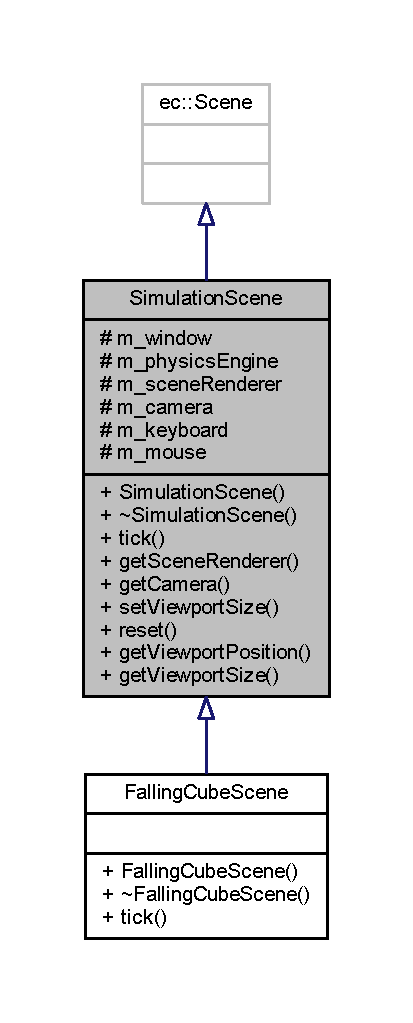
\includegraphics[width=198pt]{class_simulation_scene__inherit__graph}
\end{center}
\end{figure}


Collaboration diagram for Simulation\+Scene\+:\nopagebreak
\begin{figure}[H]
\begin{center}
\leavevmode
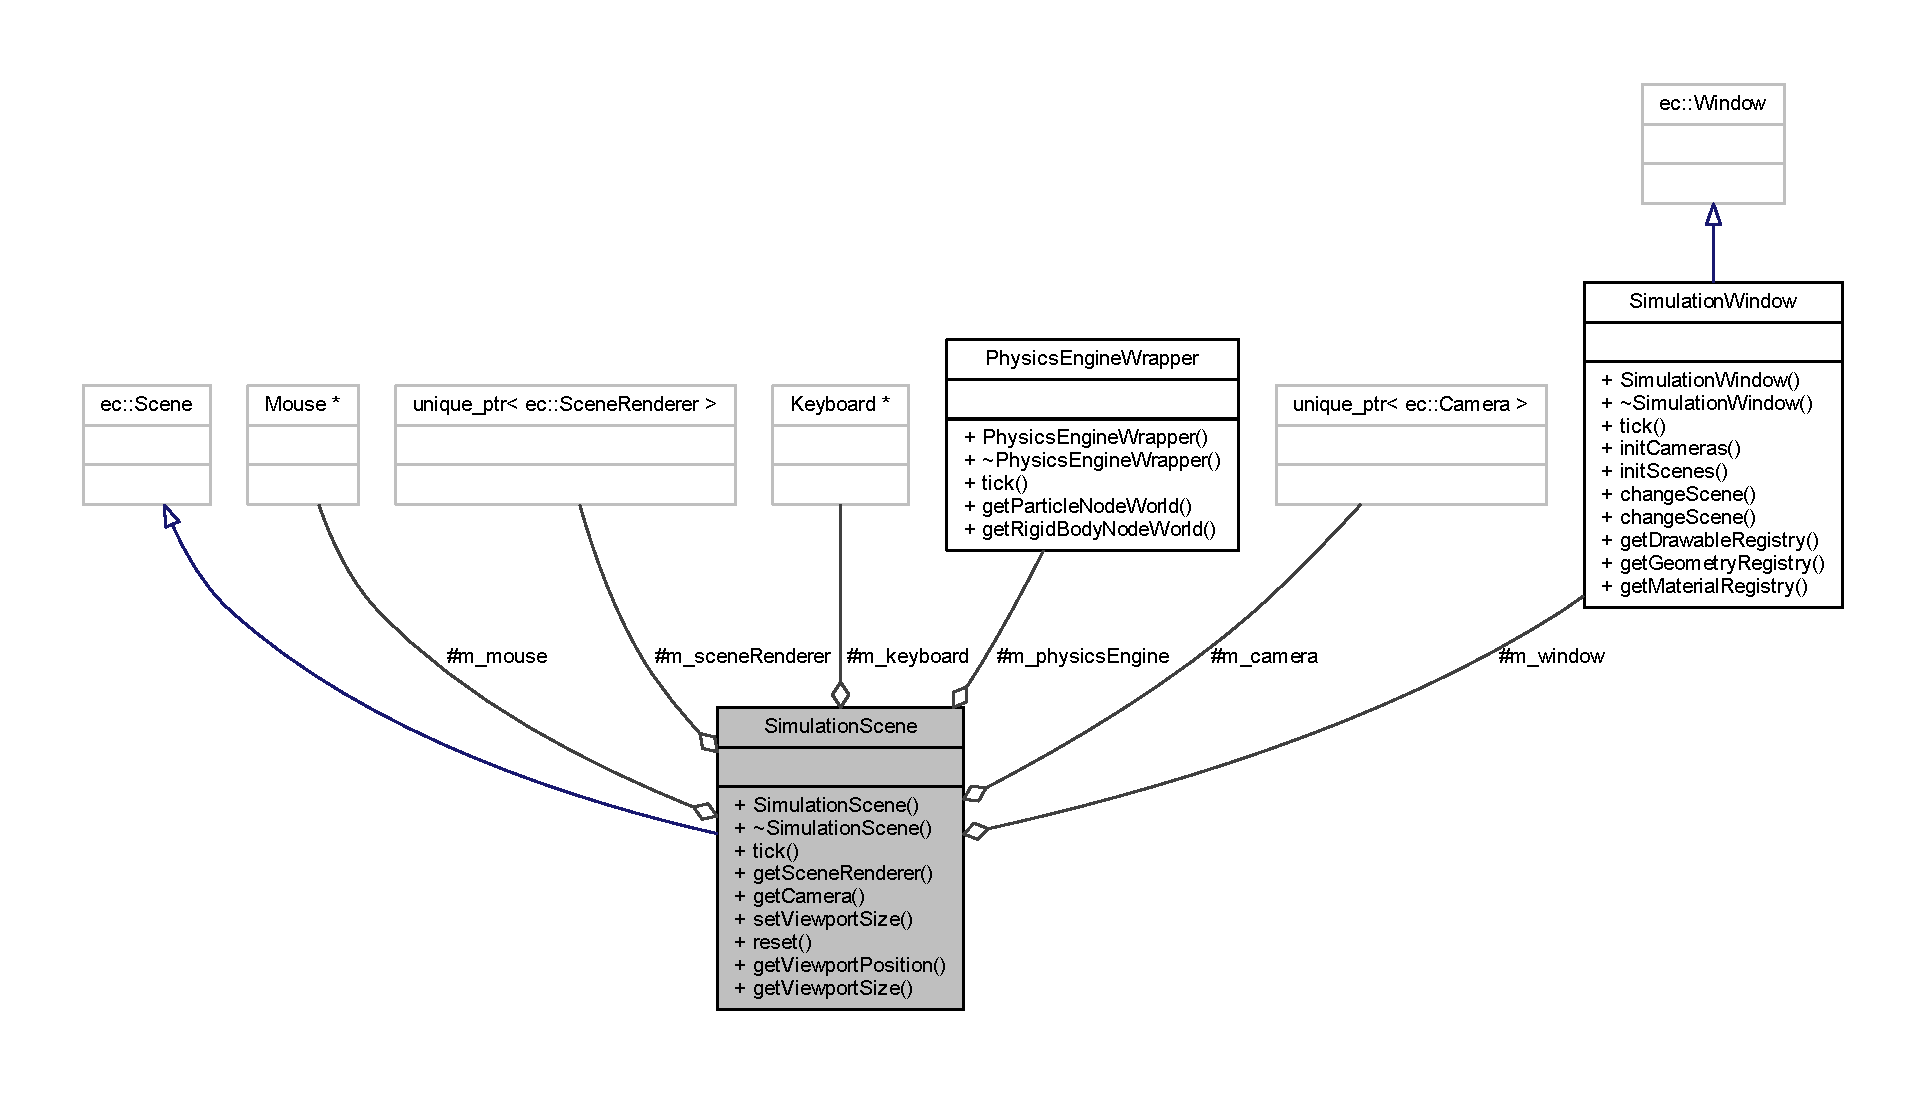
\includegraphics[width=350pt]{class_simulation_scene__coll__graph}
\end{center}
\end{figure}
\subsection*{Public Member Functions}
\begin{DoxyCompactItemize}
\item 
\mbox{\hyperlink{class_simulation_scene_a6adc5bb46c9989e666076edcb4e8e2de}{Simulation\+Scene}} (const std\+::string \&name, \mbox{\hyperlink{class_simulation_window}{Simulation\+Window}} $\ast$window)
\item 
virtual \mbox{\hyperlink{class_simulation_scene_ab084c186d269ce4576b2dda25fc0fbd6}{$\sim$\+Simulation\+Scene}} ()
\item 
void \mbox{\hyperlink{class_simulation_scene_afa830118b974cf6e579876b71ea5fb19}{tick}} (float time\+Delta) override
\item 
ec\+::\+Scene\+Renderer $\ast$ \mbox{\hyperlink{class_simulation_scene_aebc710c8b75f155eaab35f11ca825d9c}{get\+Scene\+Renderer}} () const
\item 
ec\+::\+Camera $\ast$ \mbox{\hyperlink{class_simulation_scene_a755153bde36d77afa9ad69a300463c31}{get\+Camera}} () const
\item 
void \mbox{\hyperlink{class_simulation_scene_a1a671a6caac15d53c5fbc043a58d040b}{set\+Viewport\+Size}} (const glm\+::vec2 \&size) const
\item 
virtual void \mbox{\hyperlink{class_simulation_scene_a32468fce8b00310b6e306bf558642913}{reset}} ()
\end{DoxyCompactItemize}
\subsection*{Static Public Member Functions}
\begin{DoxyCompactItemize}
\item 
static const glm\+::vec2 \& \mbox{\hyperlink{class_simulation_scene_a612b677ff28dbc9f7f6f609432ecf922}{get\+Viewport\+Position}} ()
\item 
static const glm\+::vec2 \& \mbox{\hyperlink{class_simulation_scene_a1601590e4029a75f73e46ae2bf8f24f6}{get\+Viewport\+Size}} ()
\end{DoxyCompactItemize}
\subsection*{Protected Attributes}
\begin{DoxyCompactItemize}
\item 
\mbox{\hyperlink{class_simulation_window}{Simulation\+Window}} $\ast$ \mbox{\hyperlink{class_simulation_scene_a704310f4a3436f746afcc197b0893302}{m\+\_\+window}}
\item 
\mbox{\hyperlink{class_physics_engine_wrapper}{Physics\+Engine\+Wrapper}} \mbox{\hyperlink{class_simulation_scene_aec843c805c0cad71393fe7cb18fb5c62}{m\+\_\+physics\+Engine}}
\item 
std\+::unique\+\_\+ptr$<$ ec\+::\+Scene\+Renderer $>$ \mbox{\hyperlink{class_simulation_scene_a97b314741c8056ae2168f8084926003a}{m\+\_\+scene\+Renderer}}
\item 
std\+::unique\+\_\+ptr$<$ ec\+::\+Camera $>$ \mbox{\hyperlink{class_simulation_scene_af3eac48c03330d03c304d33b21dd4d33}{m\+\_\+camera}}
\item 
ec\+::\+Keyboard $\ast$ \mbox{\hyperlink{class_simulation_scene_a8c6d930754996e9860d7ea3d63529a93}{m\+\_\+keyboard}}
\item 
ec\+::\+Mouse $\ast$ \mbox{\hyperlink{class_simulation_scene_aa48e90426a32da44796da2016a4ed10a}{m\+\_\+mouse}}
\end{DoxyCompactItemize}


\subsection{Detailed Description}
Abstract class for scenes with physic simulation. 

\subsection{Constructor \& Destructor Documentation}
\mbox{\Hypertarget{class_simulation_scene_a6adc5bb46c9989e666076edcb4e8e2de}\label{class_simulation_scene_a6adc5bb46c9989e666076edcb4e8e2de}} 
\index{Simulation\+Scene@{Simulation\+Scene}!Simulation\+Scene@{Simulation\+Scene}}
\index{Simulation\+Scene@{Simulation\+Scene}!Simulation\+Scene@{Simulation\+Scene}}
\subsubsection{\texorpdfstring{Simulation\+Scene()}{SimulationScene()}}
{\footnotesize\ttfamily Simulation\+Scene\+::\+Simulation\+Scene (\begin{DoxyParamCaption}\item[{const std\+::string \&}]{name,  }\item[{\mbox{\hyperlink{class_simulation_window}{Simulation\+Window}} $\ast$}]{window }\end{DoxyParamCaption})\hspace{0.3cm}{\ttfamily [explicit]}}

\mbox{\Hypertarget{class_simulation_scene_ab084c186d269ce4576b2dda25fc0fbd6}\label{class_simulation_scene_ab084c186d269ce4576b2dda25fc0fbd6}} 
\index{Simulation\+Scene@{Simulation\+Scene}!````~Simulation\+Scene@{$\sim$\+Simulation\+Scene}}
\index{````~Simulation\+Scene@{$\sim$\+Simulation\+Scene}!Simulation\+Scene@{Simulation\+Scene}}
\subsubsection{\texorpdfstring{$\sim$\+Simulation\+Scene()}{~SimulationScene()}}
{\footnotesize\ttfamily Simulation\+Scene\+::$\sim$\+Simulation\+Scene (\begin{DoxyParamCaption}{ }\end{DoxyParamCaption})\hspace{0.3cm}{\ttfamily [virtual]}, {\ttfamily [default]}}



\subsection{Member Function Documentation}
\mbox{\Hypertarget{class_simulation_scene_a755153bde36d77afa9ad69a300463c31}\label{class_simulation_scene_a755153bde36d77afa9ad69a300463c31}} 
\index{Simulation\+Scene@{Simulation\+Scene}!get\+Camera@{get\+Camera}}
\index{get\+Camera@{get\+Camera}!Simulation\+Scene@{Simulation\+Scene}}
\subsubsection{\texorpdfstring{get\+Camera()}{getCamera()}}
{\footnotesize\ttfamily ec\+::\+Camera $\ast$ Simulation\+Scene\+::get\+Camera (\begin{DoxyParamCaption}{ }\end{DoxyParamCaption}) const}

\mbox{\Hypertarget{class_simulation_scene_aebc710c8b75f155eaab35f11ca825d9c}\label{class_simulation_scene_aebc710c8b75f155eaab35f11ca825d9c}} 
\index{Simulation\+Scene@{Simulation\+Scene}!get\+Scene\+Renderer@{get\+Scene\+Renderer}}
\index{get\+Scene\+Renderer@{get\+Scene\+Renderer}!Simulation\+Scene@{Simulation\+Scene}}
\subsubsection{\texorpdfstring{get\+Scene\+Renderer()}{getSceneRenderer()}}
{\footnotesize\ttfamily ec\+::\+Scene\+Renderer $\ast$ Simulation\+Scene\+::get\+Scene\+Renderer (\begin{DoxyParamCaption}{ }\end{DoxyParamCaption}) const}

\mbox{\Hypertarget{class_simulation_scene_a612b677ff28dbc9f7f6f609432ecf922}\label{class_simulation_scene_a612b677ff28dbc9f7f6f609432ecf922}} 
\index{Simulation\+Scene@{Simulation\+Scene}!get\+Viewport\+Position@{get\+Viewport\+Position}}
\index{get\+Viewport\+Position@{get\+Viewport\+Position}!Simulation\+Scene@{Simulation\+Scene}}
\subsubsection{\texorpdfstring{get\+Viewport\+Position()}{getViewportPosition()}}
{\footnotesize\ttfamily const glm\+::vec2 \& Simulation\+Scene\+::get\+Viewport\+Position (\begin{DoxyParamCaption}{ }\end{DoxyParamCaption})\hspace{0.3cm}{\ttfamily [static]}}

\mbox{\Hypertarget{class_simulation_scene_a1601590e4029a75f73e46ae2bf8f24f6}\label{class_simulation_scene_a1601590e4029a75f73e46ae2bf8f24f6}} 
\index{Simulation\+Scene@{Simulation\+Scene}!get\+Viewport\+Size@{get\+Viewport\+Size}}
\index{get\+Viewport\+Size@{get\+Viewport\+Size}!Simulation\+Scene@{Simulation\+Scene}}
\subsubsection{\texorpdfstring{get\+Viewport\+Size()}{getViewportSize()}}
{\footnotesize\ttfamily const glm\+::vec2 \& Simulation\+Scene\+::get\+Viewport\+Size (\begin{DoxyParamCaption}{ }\end{DoxyParamCaption})\hspace{0.3cm}{\ttfamily [static]}}

\mbox{\Hypertarget{class_simulation_scene_a32468fce8b00310b6e306bf558642913}\label{class_simulation_scene_a32468fce8b00310b6e306bf558642913}} 
\index{Simulation\+Scene@{Simulation\+Scene}!reset@{reset}}
\index{reset@{reset}!Simulation\+Scene@{Simulation\+Scene}}
\subsubsection{\texorpdfstring{reset()}{reset()}}
{\footnotesize\ttfamily void Simulation\+Scene\+::reset (\begin{DoxyParamCaption}{ }\end{DoxyParamCaption})\hspace{0.3cm}{\ttfamily [virtual]}}

\mbox{\Hypertarget{class_simulation_scene_a1a671a6caac15d53c5fbc043a58d040b}\label{class_simulation_scene_a1a671a6caac15d53c5fbc043a58d040b}} 
\index{Simulation\+Scene@{Simulation\+Scene}!set\+Viewport\+Size@{set\+Viewport\+Size}}
\index{set\+Viewport\+Size@{set\+Viewport\+Size}!Simulation\+Scene@{Simulation\+Scene}}
\subsubsection{\texorpdfstring{set\+Viewport\+Size()}{setViewportSize()}}
{\footnotesize\ttfamily void Simulation\+Scene\+::set\+Viewport\+Size (\begin{DoxyParamCaption}\item[{const glm\+::vec2 \&}]{size }\end{DoxyParamCaption}) const}

\mbox{\Hypertarget{class_simulation_scene_afa830118b974cf6e579876b71ea5fb19}\label{class_simulation_scene_afa830118b974cf6e579876b71ea5fb19}} 
\index{Simulation\+Scene@{Simulation\+Scene}!tick@{tick}}
\index{tick@{tick}!Simulation\+Scene@{Simulation\+Scene}}
\subsubsection{\texorpdfstring{tick()}{tick()}}
{\footnotesize\ttfamily void Simulation\+Scene\+::tick (\begin{DoxyParamCaption}\item[{float}]{time\+Delta }\end{DoxyParamCaption})\hspace{0.3cm}{\ttfamily [override]}}



\subsection{Member Data Documentation}
\mbox{\Hypertarget{class_simulation_scene_af3eac48c03330d03c304d33b21dd4d33}\label{class_simulation_scene_af3eac48c03330d03c304d33b21dd4d33}} 
\index{Simulation\+Scene@{Simulation\+Scene}!m\+\_\+camera@{m\+\_\+camera}}
\index{m\+\_\+camera@{m\+\_\+camera}!Simulation\+Scene@{Simulation\+Scene}}
\subsubsection{\texorpdfstring{m\+\_\+camera}{m\_camera}}
{\footnotesize\ttfamily std\+::unique\+\_\+ptr$<$ec\+::\+Camera$>$ Simulation\+Scene\+::m\+\_\+camera\hspace{0.3cm}{\ttfamily [protected]}}

\mbox{\Hypertarget{class_simulation_scene_a8c6d930754996e9860d7ea3d63529a93}\label{class_simulation_scene_a8c6d930754996e9860d7ea3d63529a93}} 
\index{Simulation\+Scene@{Simulation\+Scene}!m\+\_\+keyboard@{m\+\_\+keyboard}}
\index{m\+\_\+keyboard@{m\+\_\+keyboard}!Simulation\+Scene@{Simulation\+Scene}}
\subsubsection{\texorpdfstring{m\+\_\+keyboard}{m\_keyboard}}
{\footnotesize\ttfamily ec\+::\+Keyboard$\ast$ Simulation\+Scene\+::m\+\_\+keyboard\hspace{0.3cm}{\ttfamily [protected]}}

\mbox{\Hypertarget{class_simulation_scene_aa48e90426a32da44796da2016a4ed10a}\label{class_simulation_scene_aa48e90426a32da44796da2016a4ed10a}} 
\index{Simulation\+Scene@{Simulation\+Scene}!m\+\_\+mouse@{m\+\_\+mouse}}
\index{m\+\_\+mouse@{m\+\_\+mouse}!Simulation\+Scene@{Simulation\+Scene}}
\subsubsection{\texorpdfstring{m\+\_\+mouse}{m\_mouse}}
{\footnotesize\ttfamily ec\+::\+Mouse$\ast$ Simulation\+Scene\+::m\+\_\+mouse\hspace{0.3cm}{\ttfamily [protected]}}

\mbox{\Hypertarget{class_simulation_scene_aec843c805c0cad71393fe7cb18fb5c62}\label{class_simulation_scene_aec843c805c0cad71393fe7cb18fb5c62}} 
\index{Simulation\+Scene@{Simulation\+Scene}!m\+\_\+physics\+Engine@{m\+\_\+physics\+Engine}}
\index{m\+\_\+physics\+Engine@{m\+\_\+physics\+Engine}!Simulation\+Scene@{Simulation\+Scene}}
\subsubsection{\texorpdfstring{m\+\_\+physics\+Engine}{m\_physicsEngine}}
{\footnotesize\ttfamily \mbox{\hyperlink{class_physics_engine_wrapper}{Physics\+Engine\+Wrapper}} Simulation\+Scene\+::m\+\_\+physics\+Engine\hspace{0.3cm}{\ttfamily [protected]}}

\mbox{\Hypertarget{class_simulation_scene_a97b314741c8056ae2168f8084926003a}\label{class_simulation_scene_a97b314741c8056ae2168f8084926003a}} 
\index{Simulation\+Scene@{Simulation\+Scene}!m\+\_\+scene\+Renderer@{m\+\_\+scene\+Renderer}}
\index{m\+\_\+scene\+Renderer@{m\+\_\+scene\+Renderer}!Simulation\+Scene@{Simulation\+Scene}}
\subsubsection{\texorpdfstring{m\+\_\+scene\+Renderer}{m\_sceneRenderer}}
{\footnotesize\ttfamily std\+::unique\+\_\+ptr$<$ec\+::\+Scene\+Renderer$>$ Simulation\+Scene\+::m\+\_\+scene\+Renderer\hspace{0.3cm}{\ttfamily [protected]}}

\mbox{\Hypertarget{class_simulation_scene_a704310f4a3436f746afcc197b0893302}\label{class_simulation_scene_a704310f4a3436f746afcc197b0893302}} 
\index{Simulation\+Scene@{Simulation\+Scene}!m\+\_\+window@{m\+\_\+window}}
\index{m\+\_\+window@{m\+\_\+window}!Simulation\+Scene@{Simulation\+Scene}}
\subsubsection{\texorpdfstring{m\+\_\+window}{m\_window}}
{\footnotesize\ttfamily \mbox{\hyperlink{class_simulation_window}{Simulation\+Window}}$\ast$ Simulation\+Scene\+::m\+\_\+window\hspace{0.3cm}{\ttfamily [protected]}}



The documentation for this class was generated from the following files\+:\begin{DoxyCompactItemize}
\item 
D\+:/\+Library/\+Documents/\+Job/\+Forschungsmaster/\+Projekte/\+Simulation\+Visualization/\+Sim/\+Sim/src/\mbox{\hyperlink{_simulation_scene_8h}{Simulation\+Scene.\+h}}\item 
D\+:/\+Library/\+Documents/\+Job/\+Forschungsmaster/\+Projekte/\+Simulation\+Visualization/\+Sim/\+Sim/src/\mbox{\hyperlink{_simulation_scene_8cpp}{Simulation\+Scene.\+cpp}}\end{DoxyCompactItemize}

\hypertarget{class_simulation_window}{}\section{Simulation\+Window Class Reference}
\label{class_simulation_window}\index{Simulation\+Window@{Simulation\+Window}}


{\ttfamily \#include $<$Simulation\+Window.\+h$>$}



Inheritance diagram for Simulation\+Window\+:\nopagebreak
\begin{figure}[H]
\begin{center}
\leavevmode
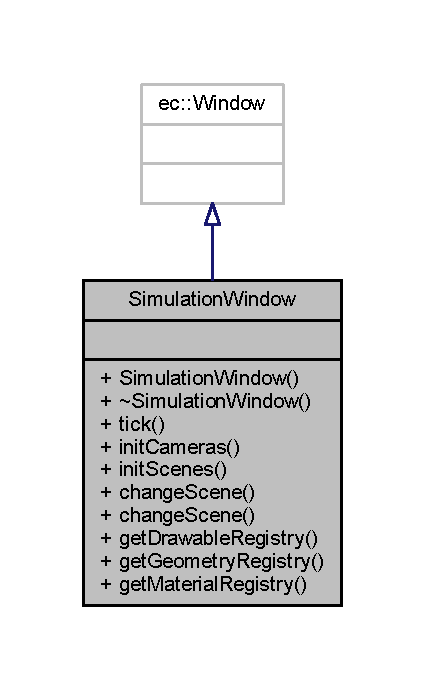
\includegraphics[width=204pt]{class_simulation_window__inherit__graph}
\end{center}
\end{figure}


Collaboration diagram for Simulation\+Window\+:\nopagebreak
\begin{figure}[H]
\begin{center}
\leavevmode
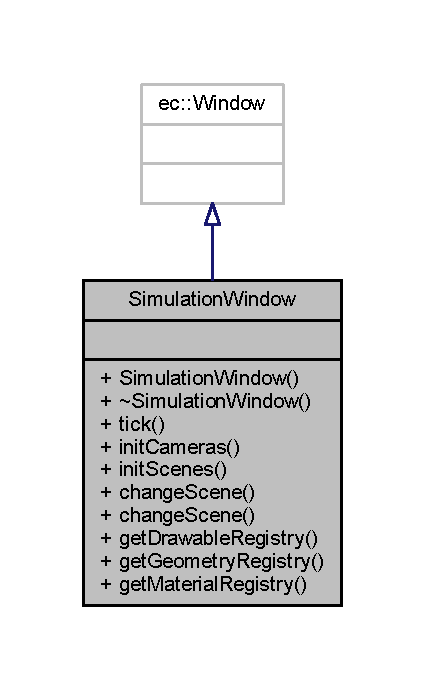
\includegraphics[width=204pt]{class_simulation_window__coll__graph}
\end{center}
\end{figure}
\subsection*{Public Member Functions}
\begin{DoxyCompactItemize}
\item 
\mbox{\hyperlink{class_simulation_window_af21a1b7626066495d16674dccd8c5fa7}{Simulation\+Window}} (unsigned int width, unsigned int height, const std\+::string \&title)
\item 
\mbox{\hyperlink{class_simulation_window_a1bad20391bd8ee4c2366bd1ac667ecdf}{$\sim$\+Simulation\+Window}} ()
\item 
void \mbox{\hyperlink{class_simulation_window_a7cde85cc846dceb4cbb9913f861b495a}{tick}} (float time\+Delta) override
\item 
void \mbox{\hyperlink{class_simulation_window_a787e405dd71c59fcf2dd58e75d233020}{init\+Cameras}} ()
\item 
void \mbox{\hyperlink{class_simulation_window_a60ebe43a626ec7acebadc93d37de8b70}{init\+Scenes}} ()
\item 
void \mbox{\hyperlink{class_simulation_window_a3f08510bb143568c18c20bd7528cb6a4}{change\+Scene}} (\mbox{\hyperlink{class_simulation_scene}{Simulation\+Scene}} $\ast$scene)
\item 
void \mbox{\hyperlink{class_simulation_window_a49e6df3f3396dbbe16dbc64c1ed7b315}{change\+Scene}} (const std\+::string \&scene\+Name)
\item 
const ec\+::\+Resource\+Registry$<$ ec\+::\+Drawable $>$ \& \mbox{\hyperlink{class_simulation_window_ae04cef316702d65cf4d6e119fa4c6cae}{get\+Drawable\+Registry}} () const
\item 
const ec\+::\+Resource\+Registry$<$ ec\+::\+Geometry $>$ \& \mbox{\hyperlink{class_simulation_window_aee0f598e5e41c2c4d8142075a294c13a}{get\+Geometry\+Registry}} () const
\item 
const ec\+::\+Resource\+Registry$<$ ec\+::\+Material $>$ \& \mbox{\hyperlink{class_simulation_window_a0be5e363792b95388f1dfae85560c5f7}{get\+Material\+Registry}} () const
\end{DoxyCompactItemize}


\subsection{Detailed Description}
This window contains a set of scenes, which we wish to simulate. It has multiple resource registries to manage materials, geometry, drawables and shaders used for visualization. 

\subsection{Constructor \& Destructor Documentation}
\mbox{\Hypertarget{class_simulation_window_af21a1b7626066495d16674dccd8c5fa7}\label{class_simulation_window_af21a1b7626066495d16674dccd8c5fa7}} 
\index{Simulation\+Window@{Simulation\+Window}!Simulation\+Window@{Simulation\+Window}}
\index{Simulation\+Window@{Simulation\+Window}!Simulation\+Window@{Simulation\+Window}}
\subsubsection{\texorpdfstring{Simulation\+Window()}{SimulationWindow()}}
{\footnotesize\ttfamily Simulation\+Window\+::\+Simulation\+Window (\begin{DoxyParamCaption}\item[{unsigned int}]{width,  }\item[{unsigned int}]{height,  }\item[{const std\+::string \&}]{title }\end{DoxyParamCaption})\hspace{0.3cm}{\ttfamily [explicit]}}

\mbox{\Hypertarget{class_simulation_window_a1bad20391bd8ee4c2366bd1ac667ecdf}\label{class_simulation_window_a1bad20391bd8ee4c2366bd1ac667ecdf}} 
\index{Simulation\+Window@{Simulation\+Window}!````~Simulation\+Window@{$\sim$\+Simulation\+Window}}
\index{````~Simulation\+Window@{$\sim$\+Simulation\+Window}!Simulation\+Window@{Simulation\+Window}}
\subsubsection{\texorpdfstring{$\sim$\+Simulation\+Window()}{~SimulationWindow()}}
{\footnotesize\ttfamily Simulation\+Window\+::$\sim$\+Simulation\+Window (\begin{DoxyParamCaption}{ }\end{DoxyParamCaption})\hspace{0.3cm}{\ttfamily [default]}}



\subsection{Member Function Documentation}
\mbox{\Hypertarget{class_simulation_window_a3f08510bb143568c18c20bd7528cb6a4}\label{class_simulation_window_a3f08510bb143568c18c20bd7528cb6a4}} 
\index{Simulation\+Window@{Simulation\+Window}!change\+Scene@{change\+Scene}}
\index{change\+Scene@{change\+Scene}!Simulation\+Window@{Simulation\+Window}}
\subsubsection{\texorpdfstring{change\+Scene()}{changeScene()}\hspace{0.1cm}{\footnotesize\ttfamily [1/2]}}
{\footnotesize\ttfamily void Simulation\+Window\+::change\+Scene (\begin{DoxyParamCaption}\item[{\mbox{\hyperlink{class_simulation_scene}{Simulation\+Scene}} $\ast$}]{scene }\end{DoxyParamCaption})}

Change the currently viewed scene. \mbox{\Hypertarget{class_simulation_window_a49e6df3f3396dbbe16dbc64c1ed7b315}\label{class_simulation_window_a49e6df3f3396dbbe16dbc64c1ed7b315}} 
\index{Simulation\+Window@{Simulation\+Window}!change\+Scene@{change\+Scene}}
\index{change\+Scene@{change\+Scene}!Simulation\+Window@{Simulation\+Window}}
\subsubsection{\texorpdfstring{change\+Scene()}{changeScene()}\hspace{0.1cm}{\footnotesize\ttfamily [2/2]}}
{\footnotesize\ttfamily void Simulation\+Window\+::change\+Scene (\begin{DoxyParamCaption}\item[{const std\+::string \&}]{scene\+Name }\end{DoxyParamCaption})}

Change the currently viewed scene. \mbox{\Hypertarget{class_simulation_window_ae04cef316702d65cf4d6e119fa4c6cae}\label{class_simulation_window_ae04cef316702d65cf4d6e119fa4c6cae}} 
\index{Simulation\+Window@{Simulation\+Window}!get\+Drawable\+Registry@{get\+Drawable\+Registry}}
\index{get\+Drawable\+Registry@{get\+Drawable\+Registry}!Simulation\+Window@{Simulation\+Window}}
\subsubsection{\texorpdfstring{get\+Drawable\+Registry()}{getDrawableRegistry()}}
{\footnotesize\ttfamily const ec\+::\+Resource\+Registry$<$ ec\+::\+Drawable $>$ \& Simulation\+Window\+::get\+Drawable\+Registry (\begin{DoxyParamCaption}{ }\end{DoxyParamCaption}) const}

Get the drawable registry. \mbox{\Hypertarget{class_simulation_window_aee0f598e5e41c2c4d8142075a294c13a}\label{class_simulation_window_aee0f598e5e41c2c4d8142075a294c13a}} 
\index{Simulation\+Window@{Simulation\+Window}!get\+Geometry\+Registry@{get\+Geometry\+Registry}}
\index{get\+Geometry\+Registry@{get\+Geometry\+Registry}!Simulation\+Window@{Simulation\+Window}}
\subsubsection{\texorpdfstring{get\+Geometry\+Registry()}{getGeometryRegistry()}}
{\footnotesize\ttfamily const ec\+::\+Resource\+Registry$<$ ec\+::\+Geometry $>$ \& Simulation\+Window\+::get\+Geometry\+Registry (\begin{DoxyParamCaption}{ }\end{DoxyParamCaption}) const}

Get the geometry registry. \mbox{\Hypertarget{class_simulation_window_a0be5e363792b95388f1dfae85560c5f7}\label{class_simulation_window_a0be5e363792b95388f1dfae85560c5f7}} 
\index{Simulation\+Window@{Simulation\+Window}!get\+Material\+Registry@{get\+Material\+Registry}}
\index{get\+Material\+Registry@{get\+Material\+Registry}!Simulation\+Window@{Simulation\+Window}}
\subsubsection{\texorpdfstring{get\+Material\+Registry()}{getMaterialRegistry()}}
{\footnotesize\ttfamily const ec\+::\+Resource\+Registry$<$ ec\+::\+Material $>$ \& Simulation\+Window\+::get\+Material\+Registry (\begin{DoxyParamCaption}{ }\end{DoxyParamCaption}) const}

Get the material registry. \mbox{\Hypertarget{class_simulation_window_a787e405dd71c59fcf2dd58e75d233020}\label{class_simulation_window_a787e405dd71c59fcf2dd58e75d233020}} 
\index{Simulation\+Window@{Simulation\+Window}!init\+Cameras@{init\+Cameras}}
\index{init\+Cameras@{init\+Cameras}!Simulation\+Window@{Simulation\+Window}}
\subsubsection{\texorpdfstring{init\+Cameras()}{initCameras()}}
{\footnotesize\ttfamily void Simulation\+Window\+::init\+Cameras (\begin{DoxyParamCaption}{ }\end{DoxyParamCaption})}

\mbox{\Hypertarget{class_simulation_window_a60ebe43a626ec7acebadc93d37de8b70}\label{class_simulation_window_a60ebe43a626ec7acebadc93d37de8b70}} 
\index{Simulation\+Window@{Simulation\+Window}!init\+Scenes@{init\+Scenes}}
\index{init\+Scenes@{init\+Scenes}!Simulation\+Window@{Simulation\+Window}}
\subsubsection{\texorpdfstring{init\+Scenes()}{initScenes()}}
{\footnotesize\ttfamily void Simulation\+Window\+::init\+Scenes (\begin{DoxyParamCaption}{ }\end{DoxyParamCaption})}

\mbox{\Hypertarget{class_simulation_window_a7cde85cc846dceb4cbb9913f861b495a}\label{class_simulation_window_a7cde85cc846dceb4cbb9913f861b495a}} 
\index{Simulation\+Window@{Simulation\+Window}!tick@{tick}}
\index{tick@{tick}!Simulation\+Window@{Simulation\+Window}}
\subsubsection{\texorpdfstring{tick()}{tick()}}
{\footnotesize\ttfamily void Simulation\+Window\+::tick (\begin{DoxyParamCaption}\item[{float}]{time\+Delta }\end{DoxyParamCaption})\hspace{0.3cm}{\ttfamily [override]}}



The documentation for this class was generated from the following files\+:\begin{DoxyCompactItemize}
\item 
D\+:/\+Library/\+Documents/\+Job/\+Forschungsmaster/\+Projekte/\+Simulation\+Visualization/\+Sim/\+Sim/src/\mbox{\hyperlink{_simulation_window_8h}{Simulation\+Window.\+h}}\item 
D\+:/\+Library/\+Documents/\+Job/\+Forschungsmaster/\+Projekte/\+Simulation\+Visualization/\+Sim/\+Sim/src/\mbox{\hyperlink{_simulation_window_8cpp}{Simulation\+Window.\+cpp}}\end{DoxyCompactItemize}

\chapter{File Documentation}
\hypertarget{_falling_cube_scene_8cpp}{}\section{D\+:/\+Library/\+Documents/\+Job/\+Forschungsmaster/\+Projekte/\+Simulation\+Visualization/\+Sim/\+Sim/src/\+Examples/\+Falling\+Cube\+Scene.cpp File Reference}
\label{_falling_cube_scene_8cpp}\index{D\+:/\+Library/\+Documents/\+Job/\+Forschungsmaster/\+Projekte/\+Simulation\+Visualization/\+Sim/\+Sim/src/\+Examples/\+Falling\+Cube\+Scene.\+cpp@{D\+:/\+Library/\+Documents/\+Job/\+Forschungsmaster/\+Projekte/\+Simulation\+Visualization/\+Sim/\+Sim/src/\+Examples/\+Falling\+Cube\+Scene.\+cpp}}
{\ttfamily \#include \char`\"{}Falling\+Cube\+Scene.\+h\char`\"{}}\newline
{\ttfamily \#include \char`\"{}Physic\+Interfaces/\+Particle\+Node\+World.\+h\char`\"{}}\newline
{\ttfamily \#include \char`\"{}R3\+D/\+Particle\+Engine/\+Particle\+World.\+h\char`\"{}}\newline
{\ttfamily \#include \char`\"{}E\+C3\+D/\+Core/\+Resource\+Registry.\+h\char`\"{}}\newline
{\ttfamily \#include \char`\"{}E\+C3\+D/\+Core/\+Drawable.\+h\char`\"{}}\newline
Include dependency graph for Falling\+Cube\+Scene.\+cpp\+:\nopagebreak
\begin{figure}[H]
\begin{center}
\leavevmode
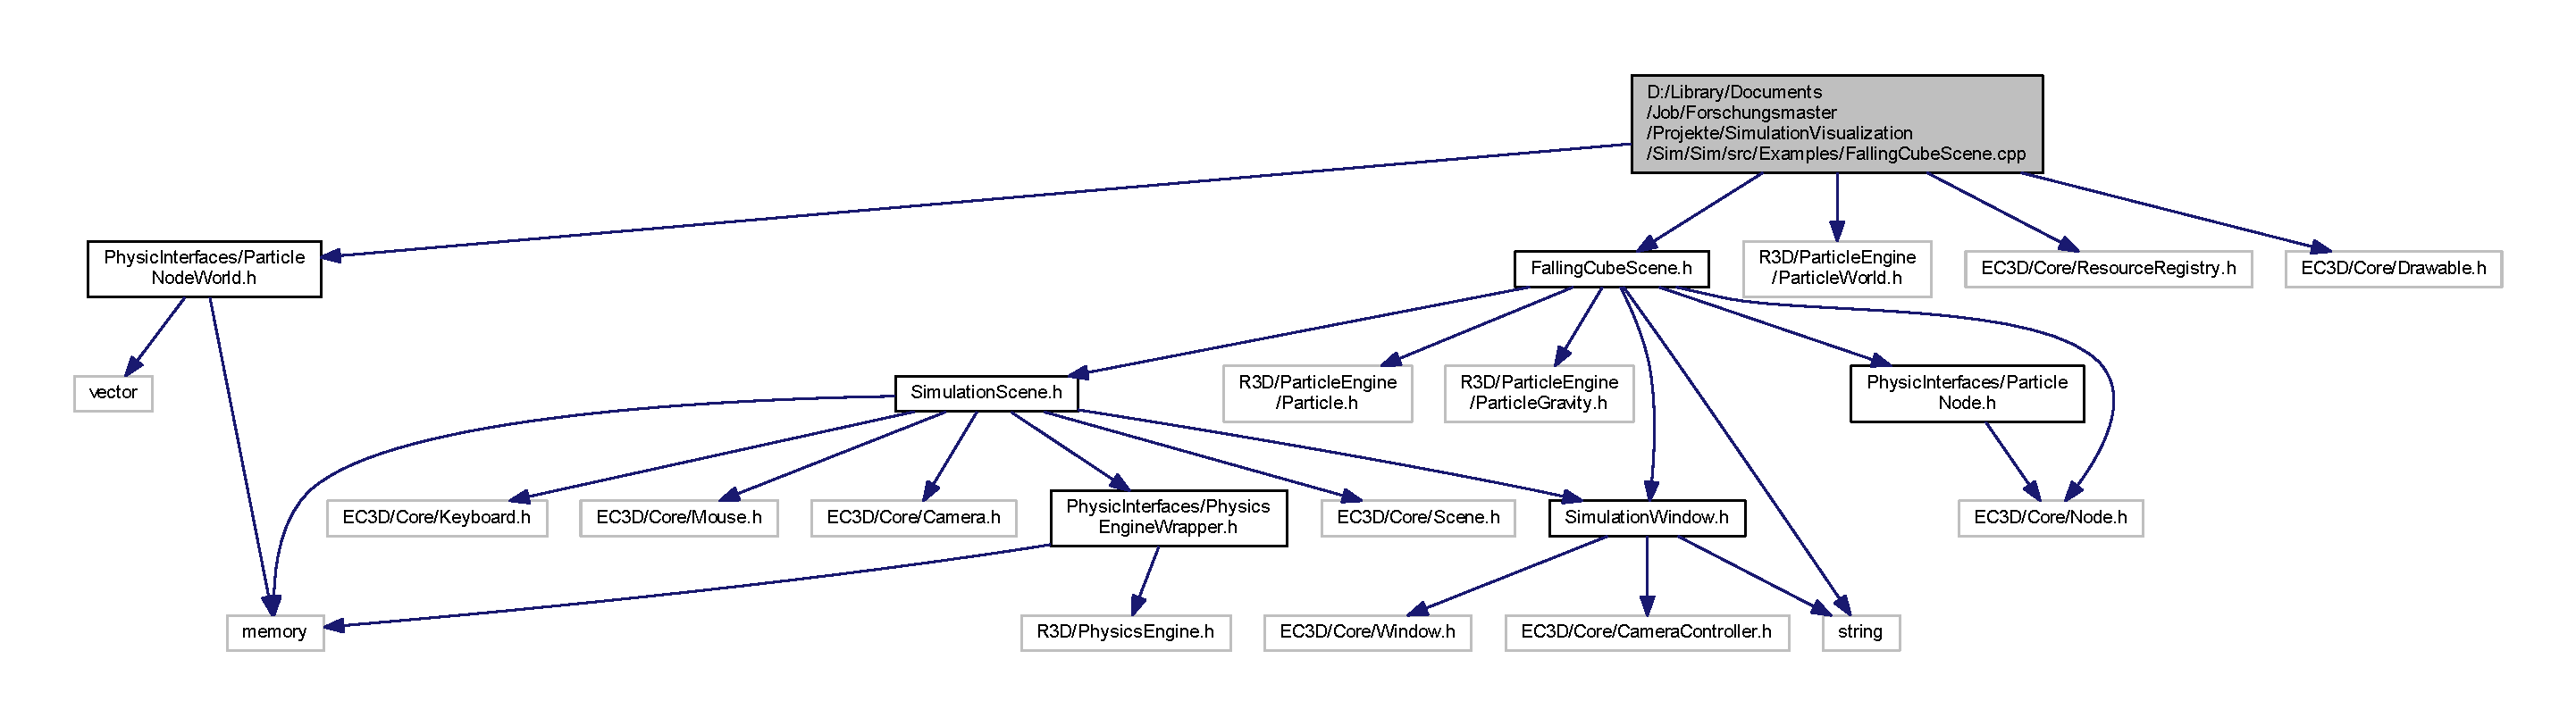
\includegraphics[width=350pt]{_falling_cube_scene_8cpp__incl}
\end{center}
\end{figure}

\hypertarget{_falling_cube_scene_8h}{}\section{D\+:/\+Library/\+Documents/\+Job/\+Forschungsmaster/\+Projekte/\+Simulation\+Visualization/\+Sim/\+Sim/src/\+Examples/\+Falling\+Cube\+Scene.h File Reference}
\label{_falling_cube_scene_8h}\index{D\+:/\+Library/\+Documents/\+Job/\+Forschungsmaster/\+Projekte/\+Simulation\+Visualization/\+Sim/\+Sim/src/\+Examples/\+Falling\+Cube\+Scene.\+h@{D\+:/\+Library/\+Documents/\+Job/\+Forschungsmaster/\+Projekte/\+Simulation\+Visualization/\+Sim/\+Sim/src/\+Examples/\+Falling\+Cube\+Scene.\+h}}
{\ttfamily \#include \char`\"{}Simulation\+Scene.\+h\char`\"{}}\newline
{\ttfamily \#include \char`\"{}Simulation\+Window.\+h\char`\"{}}\newline
{\ttfamily \#include \char`\"{}Physic\+Interfaces/\+Particle\+Node.\+h\char`\"{}}\newline
{\ttfamily \#include \char`\"{}R3\+D/\+Particle\+Engine/\+Particle.\+h\char`\"{}}\newline
{\ttfamily \#include \char`\"{}R3\+D/\+Particle\+Engine/\+Particle\+Gravity.\+h\char`\"{}}\newline
{\ttfamily \#include \char`\"{}E\+C3\+D/\+Core/\+Node.\+h\char`\"{}}\newline
{\ttfamily \#include $<$string$>$}\newline
Include dependency graph for Falling\+Cube\+Scene.\+h\+:\nopagebreak
\begin{figure}[H]
\begin{center}
\leavevmode
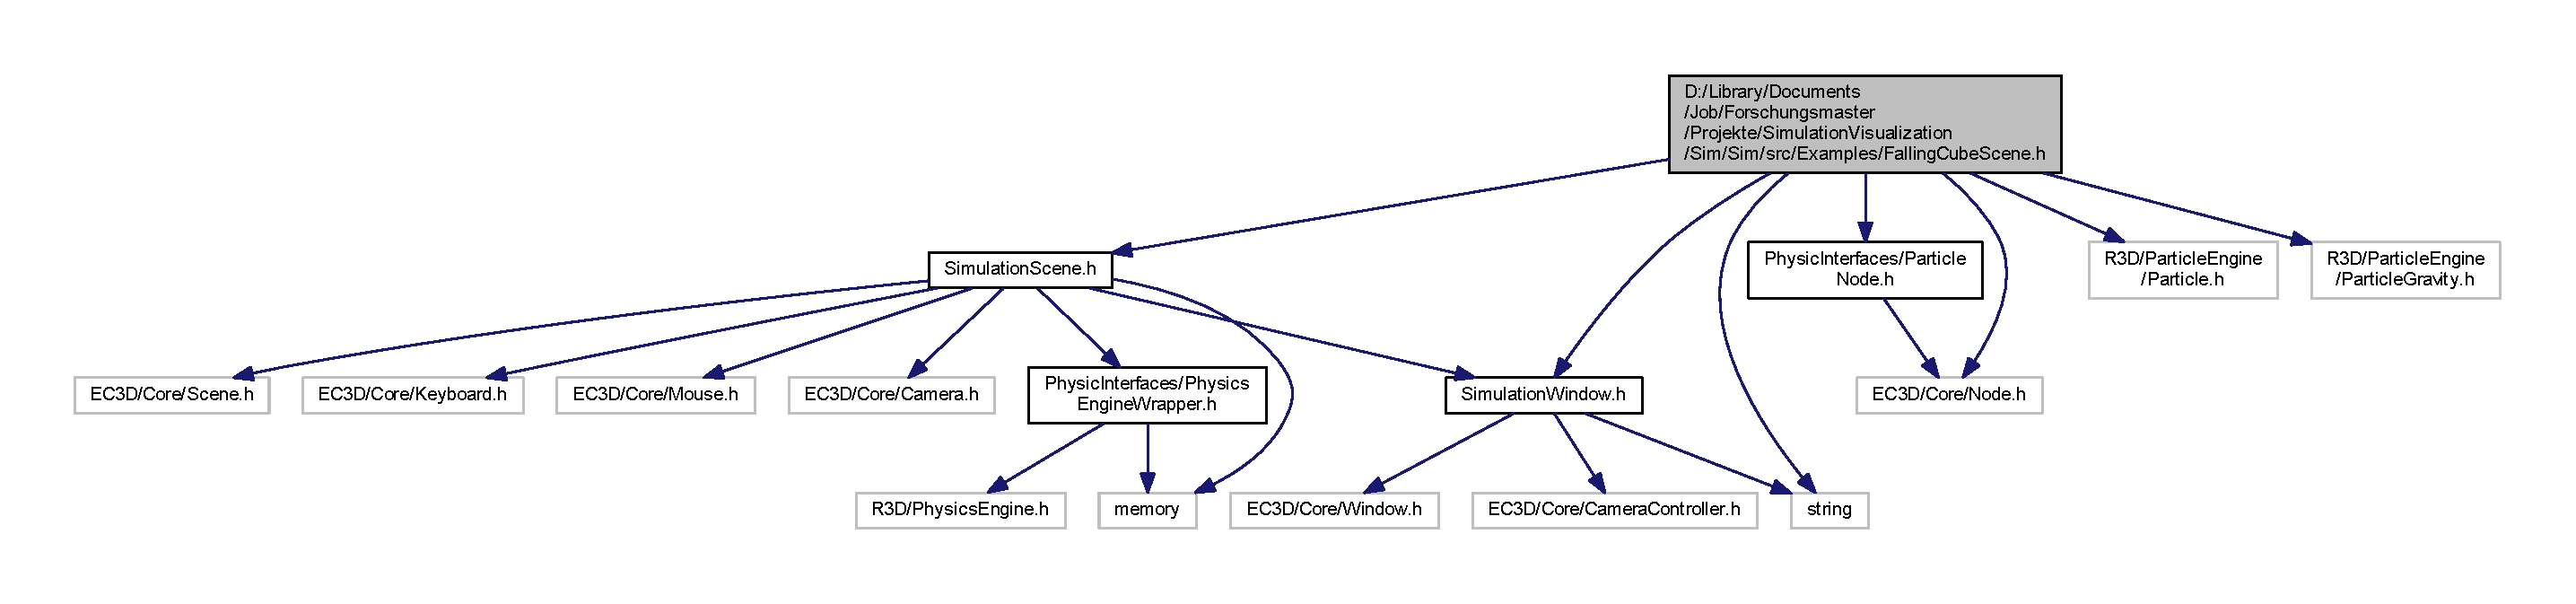
\includegraphics[width=350pt]{_falling_cube_scene_8h__incl}
\end{center}
\end{figure}
This graph shows which files directly or indirectly include this file\+:\nopagebreak
\begin{figure}[H]
\begin{center}
\leavevmode
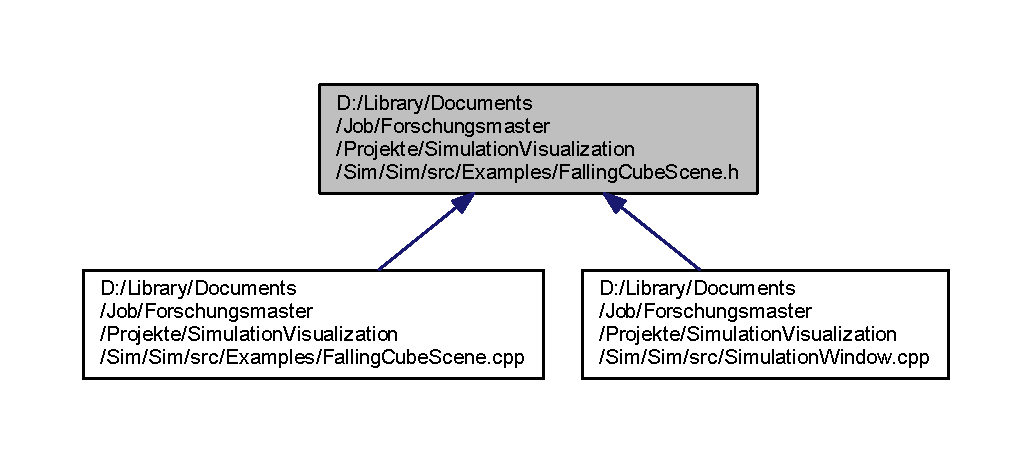
\includegraphics[width=350pt]{_falling_cube_scene_8h__dep__incl}
\end{center}
\end{figure}
\subsection*{Classes}
\begin{DoxyCompactItemize}
\item 
class \mbox{\hyperlink{class_falling_cube_scene}{Falling\+Cube\+Scene}}
\end{DoxyCompactItemize}

\hypertarget{main_8cpp}{}\section{D\+:/\+Library/\+Documents/\+Job/\+Forschungsmaster/\+Projekte/\+Simulation\+Visualization/\+Sim/\+Sim/src/main.cpp File Reference}
\label{main_8cpp}\index{D\+:/\+Library/\+Documents/\+Job/\+Forschungsmaster/\+Projekte/\+Simulation\+Visualization/\+Sim/\+Sim/src/main.\+cpp@{D\+:/\+Library/\+Documents/\+Job/\+Forschungsmaster/\+Projekte/\+Simulation\+Visualization/\+Sim/\+Sim/src/main.\+cpp}}
{\ttfamily \#include \char`\"{}Simulation\+Window.\+h\char`\"{}}\newline
{\ttfamily \#include \char`\"{}E\+C3\+D/\+Gui/\+Mini\+Agui.\+h\char`\"{}}\newline
{\ttfamily \#include \char`\"{}E\+C3\+D/\+Core/\+Application.\+h\char`\"{}}\newline
Include dependency graph for main.\+cpp\+:\nopagebreak
\begin{figure}[H]
\begin{center}
\leavevmode
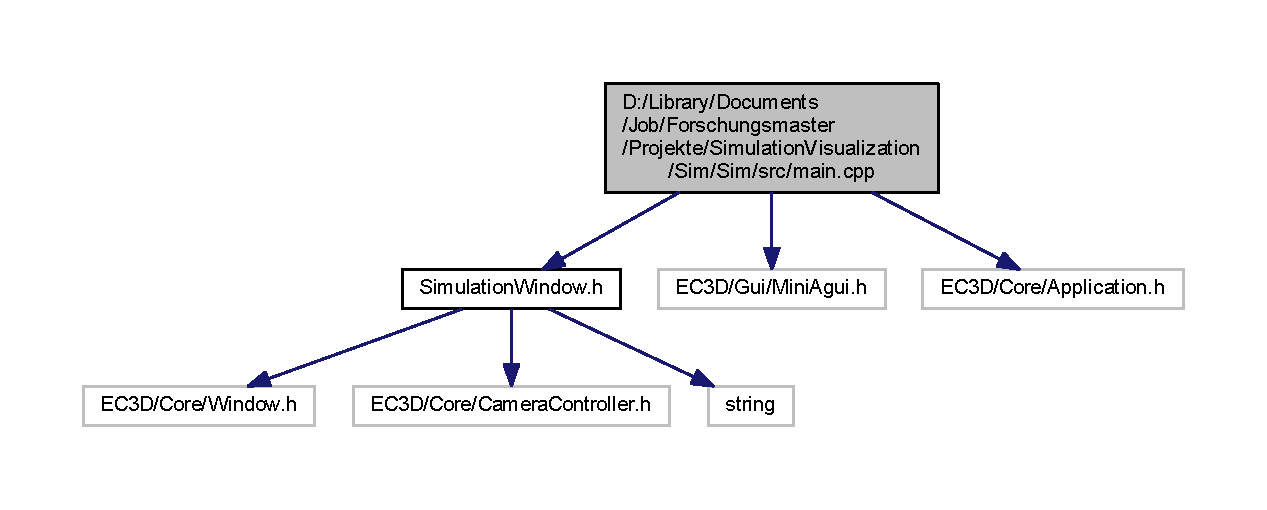
\includegraphics[width=350pt]{main_8cpp__incl}
\end{center}
\end{figure}
\subsection*{Functions}
\begin{DoxyCompactItemize}
\item 
int \mbox{\hyperlink{main_8cpp_a3c04138a5bfe5d72780bb7e82a18e627}{main}} (int argc, char $\ast$$\ast$argv)
\end{DoxyCompactItemize}


\subsection{Function Documentation}
\mbox{\Hypertarget{main_8cpp_a3c04138a5bfe5d72780bb7e82a18e627}\label{main_8cpp_a3c04138a5bfe5d72780bb7e82a18e627}} 
\index{main.\+cpp@{main.\+cpp}!main@{main}}
\index{main@{main}!main.\+cpp@{main.\+cpp}}
\subsubsection{\texorpdfstring{main()}{main()}}
{\footnotesize\ttfamily int main (\begin{DoxyParamCaption}\item[{int}]{argc,  }\item[{char $\ast$$\ast$}]{argv }\end{DoxyParamCaption})}


\hypertarget{_particle_node_8cpp}{}\section{D\+:/\+Library/\+Documents/\+Job/\+Forschungsmaster/\+Projekte/\+Simulation\+Visualization/\+Sim/\+Sim/src/\+Physic\+Interfaces/\+Particle\+Node.cpp File Reference}
\label{_particle_node_8cpp}\index{D\+:/\+Library/\+Documents/\+Job/\+Forschungsmaster/\+Projekte/\+Simulation\+Visualization/\+Sim/\+Sim/src/\+Physic\+Interfaces/\+Particle\+Node.\+cpp@{D\+:/\+Library/\+Documents/\+Job/\+Forschungsmaster/\+Projekte/\+Simulation\+Visualization/\+Sim/\+Sim/src/\+Physic\+Interfaces/\+Particle\+Node.\+cpp}}
{\ttfamily \#include \char`\"{}Particle\+Node.\+h\char`\"{}}\newline
{\ttfamily \#include \char`\"{}R3\+D/\+Particle\+Engine/\+Particle.\+h\char`\"{}}\newline
Include dependency graph for Particle\+Node.\+cpp\+:\nopagebreak
\begin{figure}[H]
\begin{center}
\leavevmode
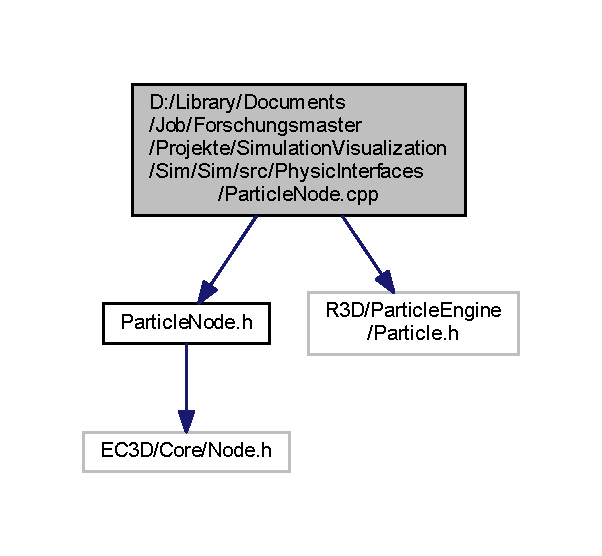
\includegraphics[width=289pt]{_particle_node_8cpp__incl}
\end{center}
\end{figure}

\hypertarget{_particle_node_8h}{}\section{D\+:/\+Library/\+Documents/\+Job/\+Forschungsmaster/\+Projekte/\+Simulation\+Visualization/\+Sim/\+Sim/src/\+Physic\+Interfaces/\+Particle\+Node.h File Reference}
\label{_particle_node_8h}\index{D\+:/\+Library/\+Documents/\+Job/\+Forschungsmaster/\+Projekte/\+Simulation\+Visualization/\+Sim/\+Sim/src/\+Physic\+Interfaces/\+Particle\+Node.\+h@{D\+:/\+Library/\+Documents/\+Job/\+Forschungsmaster/\+Projekte/\+Simulation\+Visualization/\+Sim/\+Sim/src/\+Physic\+Interfaces/\+Particle\+Node.\+h}}
{\ttfamily \#include \char`\"{}E\+C3\+D/\+Core/\+Node.\+h\char`\"{}}\newline
Include dependency graph for Particle\+Node.\+h\+:\nopagebreak
\begin{figure}[H]
\begin{center}
\leavevmode
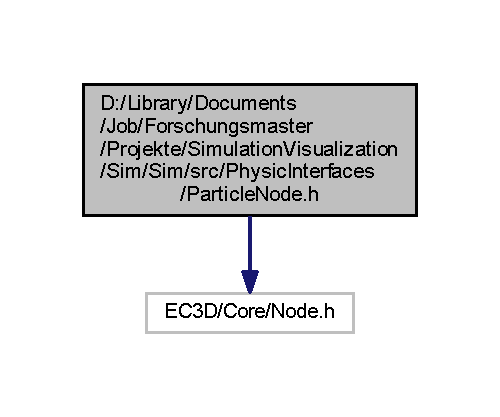
\includegraphics[width=240pt]{_particle_node_8h__incl}
\end{center}
\end{figure}
This graph shows which files directly or indirectly include this file\+:\nopagebreak
\begin{figure}[H]
\begin{center}
\leavevmode
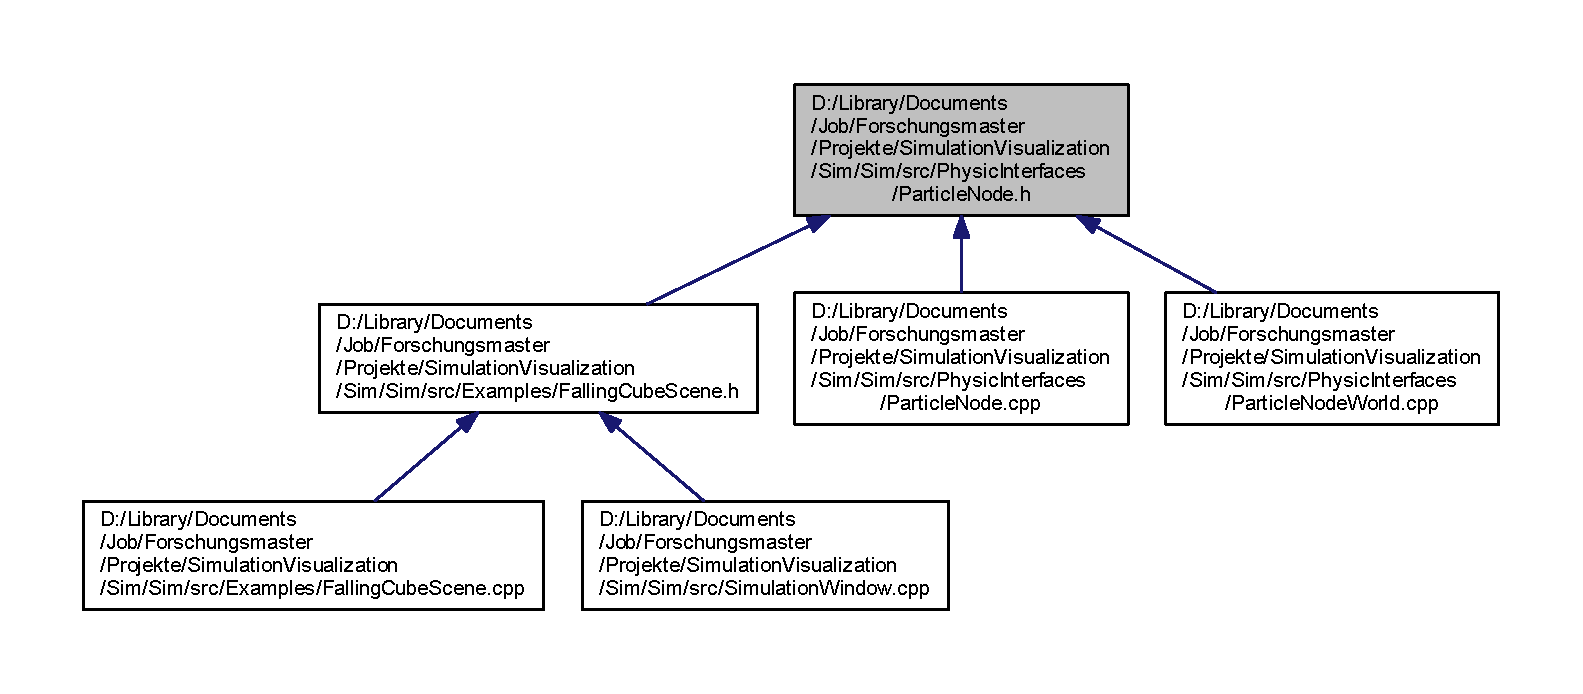
\includegraphics[width=350pt]{_particle_node_8h__dep__incl}
\end{center}
\end{figure}
\subsection*{Classes}
\begin{DoxyCompactItemize}
\item 
class \mbox{\hyperlink{class_particle_node}{Particle\+Node}}
\end{DoxyCompactItemize}
\subsection*{Namespaces}
\begin{DoxyCompactItemize}
\item 
 \mbox{\hyperlink{namespacer3}{r3}}
\end{DoxyCompactItemize}

\hypertarget{_particle_node_world_8cpp}{}\section{D\+:/\+Library/\+Documents/\+Job/\+Forschungsmaster/\+Projekte/\+Simulation\+Visualization/\+Sim/\+Sim/src/\+Physic\+Interfaces/\+Particle\+Node\+World.cpp File Reference}
\label{_particle_node_world_8cpp}\index{D\+:/\+Library/\+Documents/\+Job/\+Forschungsmaster/\+Projekte/\+Simulation\+Visualization/\+Sim/\+Sim/src/\+Physic\+Interfaces/\+Particle\+Node\+World.\+cpp@{D\+:/\+Library/\+Documents/\+Job/\+Forschungsmaster/\+Projekte/\+Simulation\+Visualization/\+Sim/\+Sim/src/\+Physic\+Interfaces/\+Particle\+Node\+World.\+cpp}}
{\ttfamily \#include \char`\"{}Particle\+Node\+World.\+h\char`\"{}}\newline
{\ttfamily \#include \char`\"{}R3\+D/\+Particle\+Engine/\+Particle\+World.\+h\char`\"{}}\newline
{\ttfamily \#include \char`\"{}R3\+D/\+Particle\+Engine/\+Default\+Particle\+Engine\+C\+I.\+h\char`\"{}}\newline
{\ttfamily \#include \char`\"{}Particle\+Node.\+h\char`\"{}}\newline
{\ttfamily \#include $<$algorithm$>$}\newline
Include dependency graph for Particle\+Node\+World.\+cpp\+:\nopagebreak
\begin{figure}[H]
\begin{center}
\leavevmode
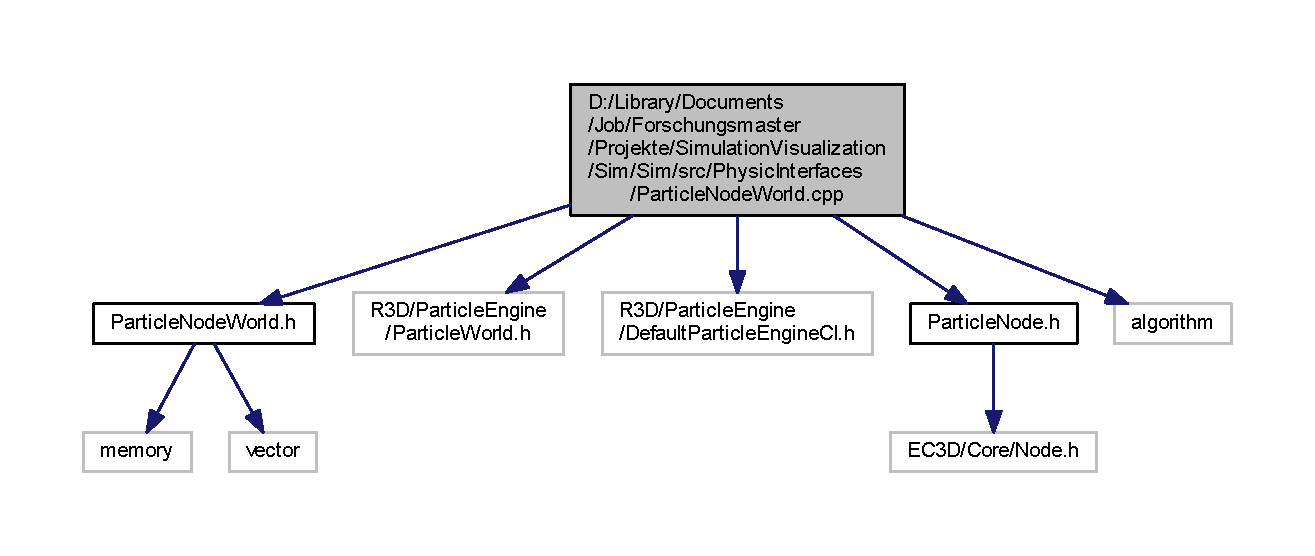
\includegraphics[width=350pt]{_particle_node_world_8cpp__incl}
\end{center}
\end{figure}

\hypertarget{_particle_node_world_8h}{}\section{D\+:/\+Library/\+Documents/\+Job/\+Forschungsmaster/\+Projekte/\+Simulation\+Visualization/\+Sim/\+Sim/src/\+Physic\+Interfaces/\+Particle\+Node\+World.h File Reference}
\label{_particle_node_world_8h}\index{D\+:/\+Library/\+Documents/\+Job/\+Forschungsmaster/\+Projekte/\+Simulation\+Visualization/\+Sim/\+Sim/src/\+Physic\+Interfaces/\+Particle\+Node\+World.\+h@{D\+:/\+Library/\+Documents/\+Job/\+Forschungsmaster/\+Projekte/\+Simulation\+Visualization/\+Sim/\+Sim/src/\+Physic\+Interfaces/\+Particle\+Node\+World.\+h}}
{\ttfamily \#include $<$memory$>$}\newline
{\ttfamily \#include $<$vector$>$}\newline
Include dependency graph for Particle\+Node\+World.\+h\+:\nopagebreak
\begin{figure}[H]
\begin{center}
\leavevmode
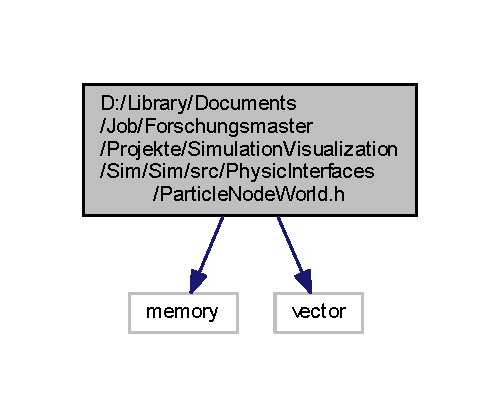
\includegraphics[width=240pt]{_particle_node_world_8h__incl}
\end{center}
\end{figure}
This graph shows which files directly or indirectly include this file\+:\nopagebreak
\begin{figure}[H]
\begin{center}
\leavevmode
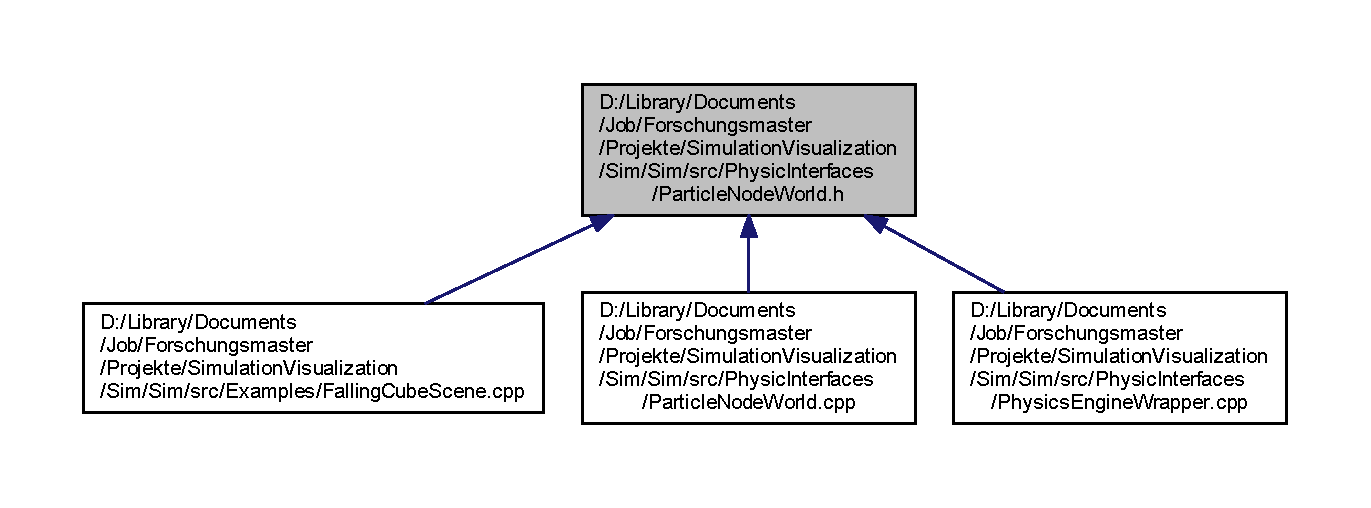
\includegraphics[width=350pt]{_particle_node_world_8h__dep__incl}
\end{center}
\end{figure}
\subsection*{Classes}
\begin{DoxyCompactItemize}
\item 
class \mbox{\hyperlink{class_particle_node_world}{Particle\+Node\+World}}
\end{DoxyCompactItemize}
\subsection*{Namespaces}
\begin{DoxyCompactItemize}
\item 
 \mbox{\hyperlink{namespacer3}{r3}}
\end{DoxyCompactItemize}

\hypertarget{_physics_engine_wrapper_8cpp}{}\section{D\+:/\+Library/\+Documents/\+Job/\+Forschungsmaster/\+Projekte/\+Simulation\+Visualization/\+Sim/\+Sim/src/\+Physic\+Interfaces/\+Physics\+Engine\+Wrapper.cpp File Reference}
\label{_physics_engine_wrapper_8cpp}\index{D\+:/\+Library/\+Documents/\+Job/\+Forschungsmaster/\+Projekte/\+Simulation\+Visualization/\+Sim/\+Sim/src/\+Physic\+Interfaces/\+Physics\+Engine\+Wrapper.\+cpp@{D\+:/\+Library/\+Documents/\+Job/\+Forschungsmaster/\+Projekte/\+Simulation\+Visualization/\+Sim/\+Sim/src/\+Physic\+Interfaces/\+Physics\+Engine\+Wrapper.\+cpp}}
{\ttfamily \#include \char`\"{}Physics\+Engine\+Wrapper.\+h\char`\"{}}\newline
{\ttfamily \#include \char`\"{}R3\+D/\+Particle\+Engine/\+Particle\+World.\+h\char`\"{}}\newline
{\ttfamily \#include \char`\"{}R3\+D/\+Rigid\+Body\+Engine/\+Rigid\+Body\+World.\+h\char`\"{}}\newline
{\ttfamily \#include \char`\"{}Particle\+Node\+World.\+h\char`\"{}}\newline
{\ttfamily \#include \char`\"{}Rigid\+Body\+Node\+World.\+h\char`\"{}}\newline
Include dependency graph for Physics\+Engine\+Wrapper.\+cpp\+:\nopagebreak
\begin{figure}[H]
\begin{center}
\leavevmode
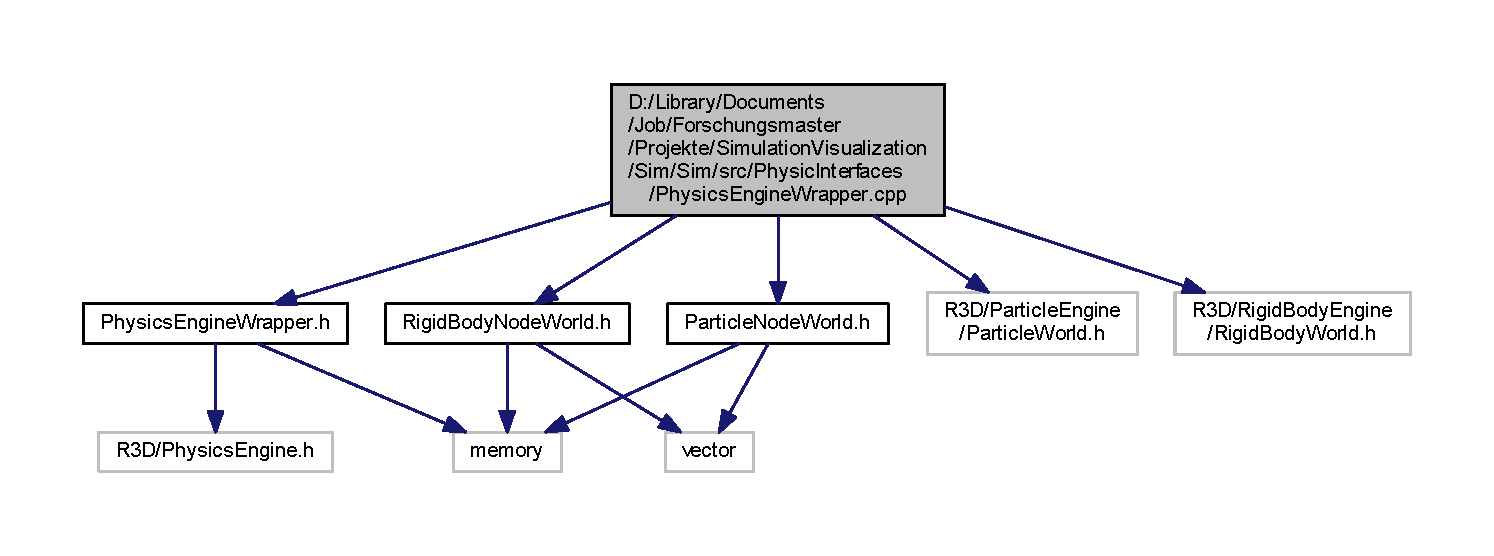
\includegraphics[width=350pt]{_physics_engine_wrapper_8cpp__incl}
\end{center}
\end{figure}

\hypertarget{_physics_engine_wrapper_8h}{}\section{D\+:/\+Library/\+Documents/\+Job/\+Forschungsmaster/\+Projekte/\+Simulation\+Visualization/\+Sim/\+Sim/src/\+Physic\+Interfaces/\+Physics\+Engine\+Wrapper.h File Reference}
\label{_physics_engine_wrapper_8h}\index{D\+:/\+Library/\+Documents/\+Job/\+Forschungsmaster/\+Projekte/\+Simulation\+Visualization/\+Sim/\+Sim/src/\+Physic\+Interfaces/\+Physics\+Engine\+Wrapper.\+h@{D\+:/\+Library/\+Documents/\+Job/\+Forschungsmaster/\+Projekte/\+Simulation\+Visualization/\+Sim/\+Sim/src/\+Physic\+Interfaces/\+Physics\+Engine\+Wrapper.\+h}}
{\ttfamily \#include \char`\"{}R3\+D/\+Physics\+Engine.\+h\char`\"{}}\newline
{\ttfamily \#include $<$memory$>$}\newline
Include dependency graph for Physics\+Engine\+Wrapper.\+h\+:\nopagebreak
\begin{figure}[H]
\begin{center}
\leavevmode
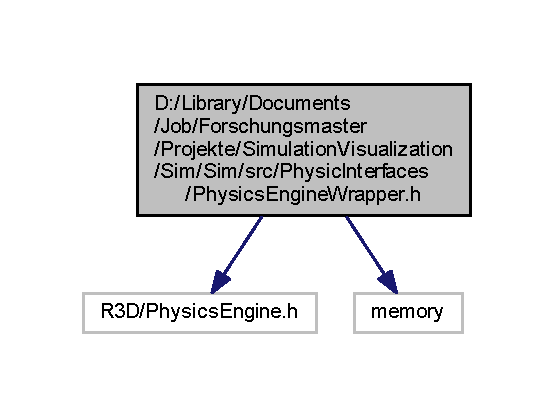
\includegraphics[width=266pt]{_physics_engine_wrapper_8h__incl}
\end{center}
\end{figure}
This graph shows which files directly or indirectly include this file\+:\nopagebreak
\begin{figure}[H]
\begin{center}
\leavevmode
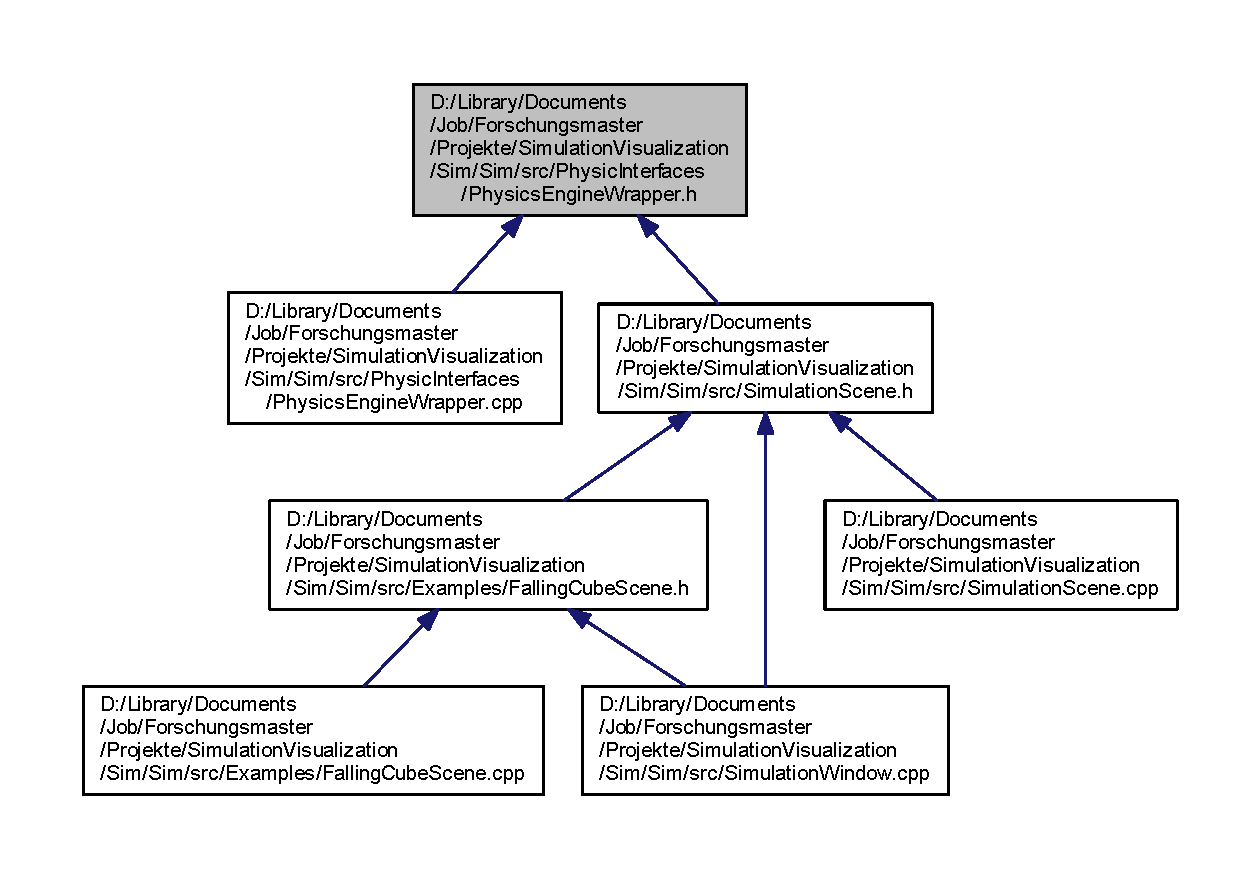
\includegraphics[width=350pt]{_physics_engine_wrapper_8h__dep__incl}
\end{center}
\end{figure}
\subsection*{Classes}
\begin{DoxyCompactItemize}
\item 
class \mbox{\hyperlink{class_physics_engine_wrapper}{Physics\+Engine\+Wrapper}}
\end{DoxyCompactItemize}

\hypertarget{_rigid_body_node_8cpp}{}\section{D\+:/\+Library/\+Documents/\+Job/\+Forschungsmaster/\+Projekte/\+Simulation\+Visualization/\+Sim/\+Sim/src/\+Physic\+Interfaces/\+Rigid\+Body\+Node.cpp File Reference}
\label{_rigid_body_node_8cpp}\index{D\+:/\+Library/\+Documents/\+Job/\+Forschungsmaster/\+Projekte/\+Simulation\+Visualization/\+Sim/\+Sim/src/\+Physic\+Interfaces/\+Rigid\+Body\+Node.\+cpp@{D\+:/\+Library/\+Documents/\+Job/\+Forschungsmaster/\+Projekte/\+Simulation\+Visualization/\+Sim/\+Sim/src/\+Physic\+Interfaces/\+Rigid\+Body\+Node.\+cpp}}
{\ttfamily \#include \char`\"{}Rigid\+Body\+Node.\+h\char`\"{}}\newline
Include dependency graph for Rigid\+Body\+Node.\+cpp\+:\nopagebreak
\begin{figure}[H]
\begin{center}
\leavevmode
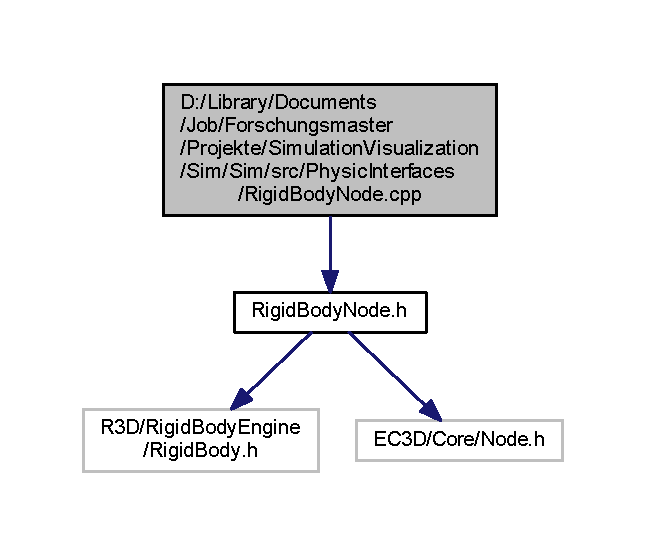
\includegraphics[width=310pt]{_rigid_body_node_8cpp__incl}
\end{center}
\end{figure}

\hypertarget{_rigid_body_node_8h}{}\section{D\+:/\+Library/\+Documents/\+Job/\+Forschungsmaster/\+Projekte/\+Simulation\+Visualization/\+Sim/\+Sim/src/\+Physic\+Interfaces/\+Rigid\+Body\+Node.h File Reference}
\label{_rigid_body_node_8h}\index{D\+:/\+Library/\+Documents/\+Job/\+Forschungsmaster/\+Projekte/\+Simulation\+Visualization/\+Sim/\+Sim/src/\+Physic\+Interfaces/\+Rigid\+Body\+Node.\+h@{D\+:/\+Library/\+Documents/\+Job/\+Forschungsmaster/\+Projekte/\+Simulation\+Visualization/\+Sim/\+Sim/src/\+Physic\+Interfaces/\+Rigid\+Body\+Node.\+h}}
{\ttfamily \#include \char`\"{}R3\+D/\+Rigid\+Body\+Engine/\+Rigid\+Body.\+h\char`\"{}}\newline
{\ttfamily \#include \char`\"{}E\+C3\+D/\+Core/\+Node.\+h\char`\"{}}\newline
Include dependency graph for Rigid\+Body\+Node.\+h\+:\nopagebreak
\begin{figure}[H]
\begin{center}
\leavevmode
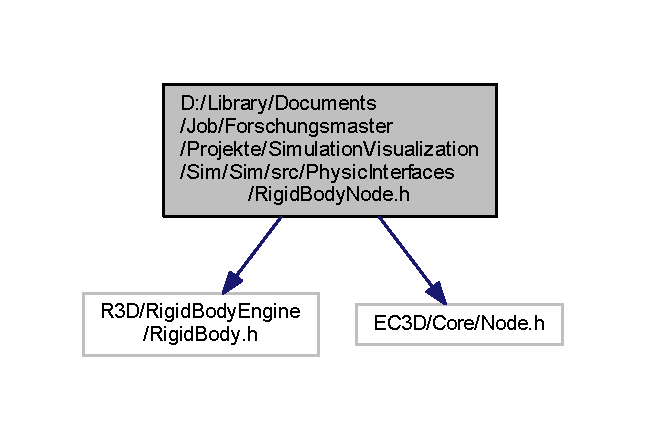
\includegraphics[width=310pt]{_rigid_body_node_8h__incl}
\end{center}
\end{figure}
This graph shows which files directly or indirectly include this file\+:\nopagebreak
\begin{figure}[H]
\begin{center}
\leavevmode
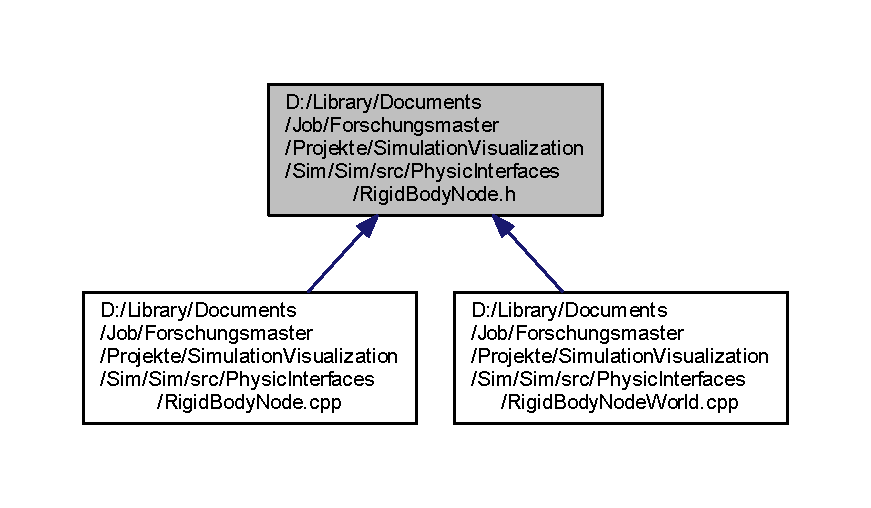
\includegraphics[width=350pt]{_rigid_body_node_8h__dep__incl}
\end{center}
\end{figure}
\subsection*{Classes}
\begin{DoxyCompactItemize}
\item 
class \mbox{\hyperlink{class_rigid_body_node}{Rigid\+Body\+Node}}
\end{DoxyCompactItemize}

\hypertarget{_rigid_body_node_world_8cpp}{}\section{D\+:/\+Library/\+Documents/\+Job/\+Forschungsmaster/\+Projekte/\+Simulation\+Visualization/\+Sim/\+Sim/src/\+Physic\+Interfaces/\+Rigid\+Body\+Node\+World.cpp File Reference}
\label{_rigid_body_node_world_8cpp}\index{D\+:/\+Library/\+Documents/\+Job/\+Forschungsmaster/\+Projekte/\+Simulation\+Visualization/\+Sim/\+Sim/src/\+Physic\+Interfaces/\+Rigid\+Body\+Node\+World.\+cpp@{D\+:/\+Library/\+Documents/\+Job/\+Forschungsmaster/\+Projekte/\+Simulation\+Visualization/\+Sim/\+Sim/src/\+Physic\+Interfaces/\+Rigid\+Body\+Node\+World.\+cpp}}
{\ttfamily \#include \char`\"{}Rigid\+Body\+Node\+World.\+h\char`\"{}}\newline
{\ttfamily \#include \char`\"{}Rigid\+Body\+Node.\+h\char`\"{}}\newline
{\ttfamily \#include \char`\"{}R3\+D/\+Rigid\+Body\+Engine/\+Rigid\+Body\+World.\+h\char`\"{}}\newline
{\ttfamily \#include \char`\"{}R3\+D/\+Rigid\+Body\+Engine/\+Default\+Rigid\+Body\+Engine\+C\+I.\+h\char`\"{}}\newline
{\ttfamily \#include $<$algorithm$>$}\newline
Include dependency graph for Rigid\+Body\+Node\+World.\+cpp\+:\nopagebreak
\begin{figure}[H]
\begin{center}
\leavevmode
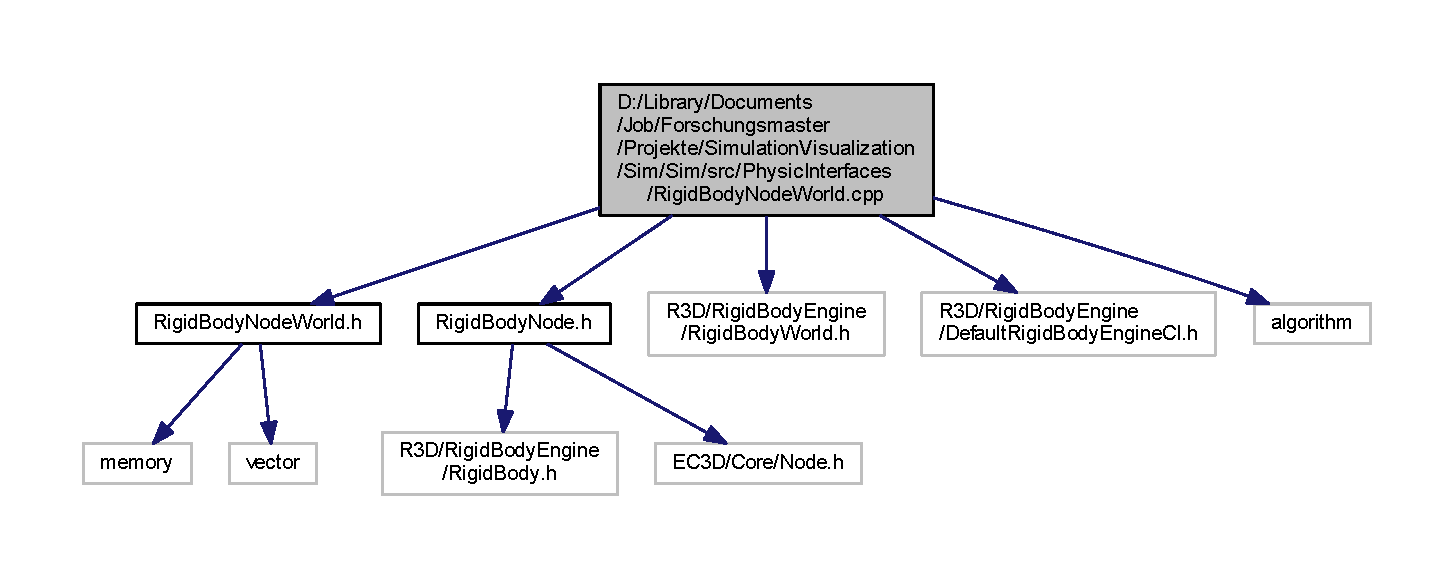
\includegraphics[width=350pt]{_rigid_body_node_world_8cpp__incl}
\end{center}
\end{figure}

\hypertarget{_rigid_body_node_world_8h}{}\section{D\+:/\+Library/\+Documents/\+Job/\+Forschungsmaster/\+Projekte/\+Simulation\+Visualization/\+Sim/\+Sim/src/\+Physic\+Interfaces/\+Rigid\+Body\+Node\+World.h File Reference}
\label{_rigid_body_node_world_8h}\index{D\+:/\+Library/\+Documents/\+Job/\+Forschungsmaster/\+Projekte/\+Simulation\+Visualization/\+Sim/\+Sim/src/\+Physic\+Interfaces/\+Rigid\+Body\+Node\+World.\+h@{D\+:/\+Library/\+Documents/\+Job/\+Forschungsmaster/\+Projekte/\+Simulation\+Visualization/\+Sim/\+Sim/src/\+Physic\+Interfaces/\+Rigid\+Body\+Node\+World.\+h}}
{\ttfamily \#include $<$memory$>$}\newline
{\ttfamily \#include $<$vector$>$}\newline
Include dependency graph for Rigid\+Body\+Node\+World.\+h\+:\nopagebreak
\begin{figure}[H]
\begin{center}
\leavevmode
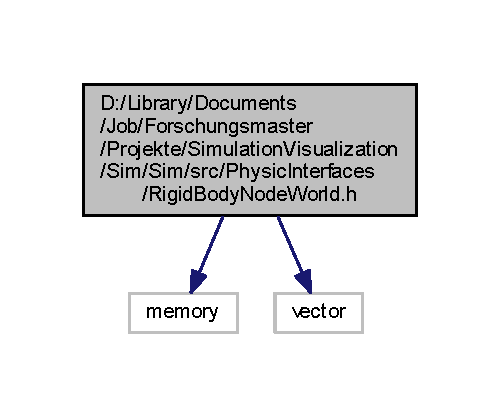
\includegraphics[width=240pt]{_rigid_body_node_world_8h__incl}
\end{center}
\end{figure}
This graph shows which files directly or indirectly include this file\+:\nopagebreak
\begin{figure}[H]
\begin{center}
\leavevmode
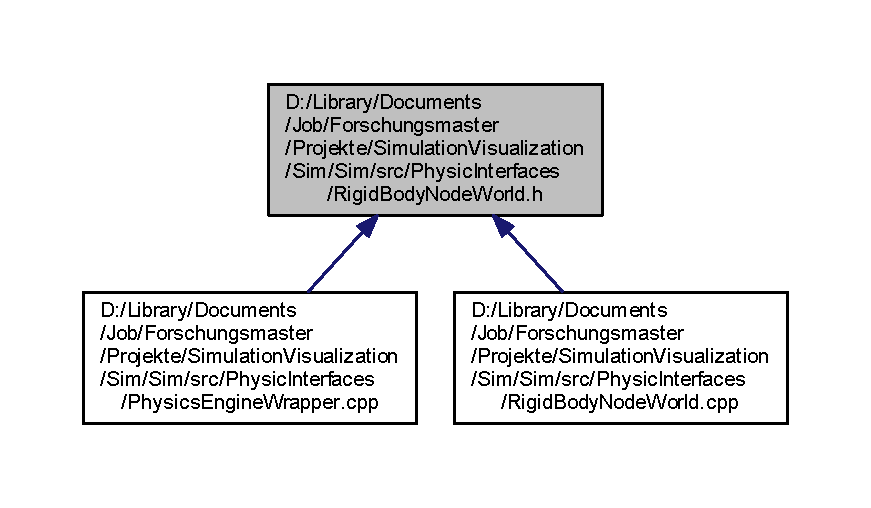
\includegraphics[width=350pt]{_rigid_body_node_world_8h__dep__incl}
\end{center}
\end{figure}
\subsection*{Classes}
\begin{DoxyCompactItemize}
\item 
class \mbox{\hyperlink{class_rigid_body_node_world}{Rigid\+Body\+Node\+World}}
\end{DoxyCompactItemize}
\subsection*{Namespaces}
\begin{DoxyCompactItemize}
\item 
 \mbox{\hyperlink{namespacer3}{r3}}
\end{DoxyCompactItemize}

\hypertarget{_simulation_scene_8cpp}{}\section{D\+:/\+Library/\+Documents/\+Job/\+Forschungsmaster/\+Projekte/\+Simulation\+Visualization/\+Sim/\+Sim/src/\+Simulation\+Scene.cpp File Reference}
\label{_simulation_scene_8cpp}\index{D\+:/\+Library/\+Documents/\+Job/\+Forschungsmaster/\+Projekte/\+Simulation\+Visualization/\+Sim/\+Sim/src/\+Simulation\+Scene.\+cpp@{D\+:/\+Library/\+Documents/\+Job/\+Forschungsmaster/\+Projekte/\+Simulation\+Visualization/\+Sim/\+Sim/src/\+Simulation\+Scene.\+cpp}}
{\ttfamily \#include \char`\"{}Simulation\+Scene.\+h\char`\"{}}\newline
{\ttfamily \#include \char`\"{}E\+C3\+D/\+Core/\+Scene\+Renderer.\+h\char`\"{}}\newline
{\ttfamily \#include \char`\"{}R3\+D/\+Rigid\+Body\+Engine/\+Rigid\+Body.\+h\char`\"{}}\newline
{\ttfamily \#include \char`\"{}R3\+D/\+Rigid\+Body\+Engine/\+Collision\+Sphere.\+h\char`\"{}}\newline
Include dependency graph for Simulation\+Scene.\+cpp\+:\nopagebreak
\begin{figure}[H]
\begin{center}
\leavevmode
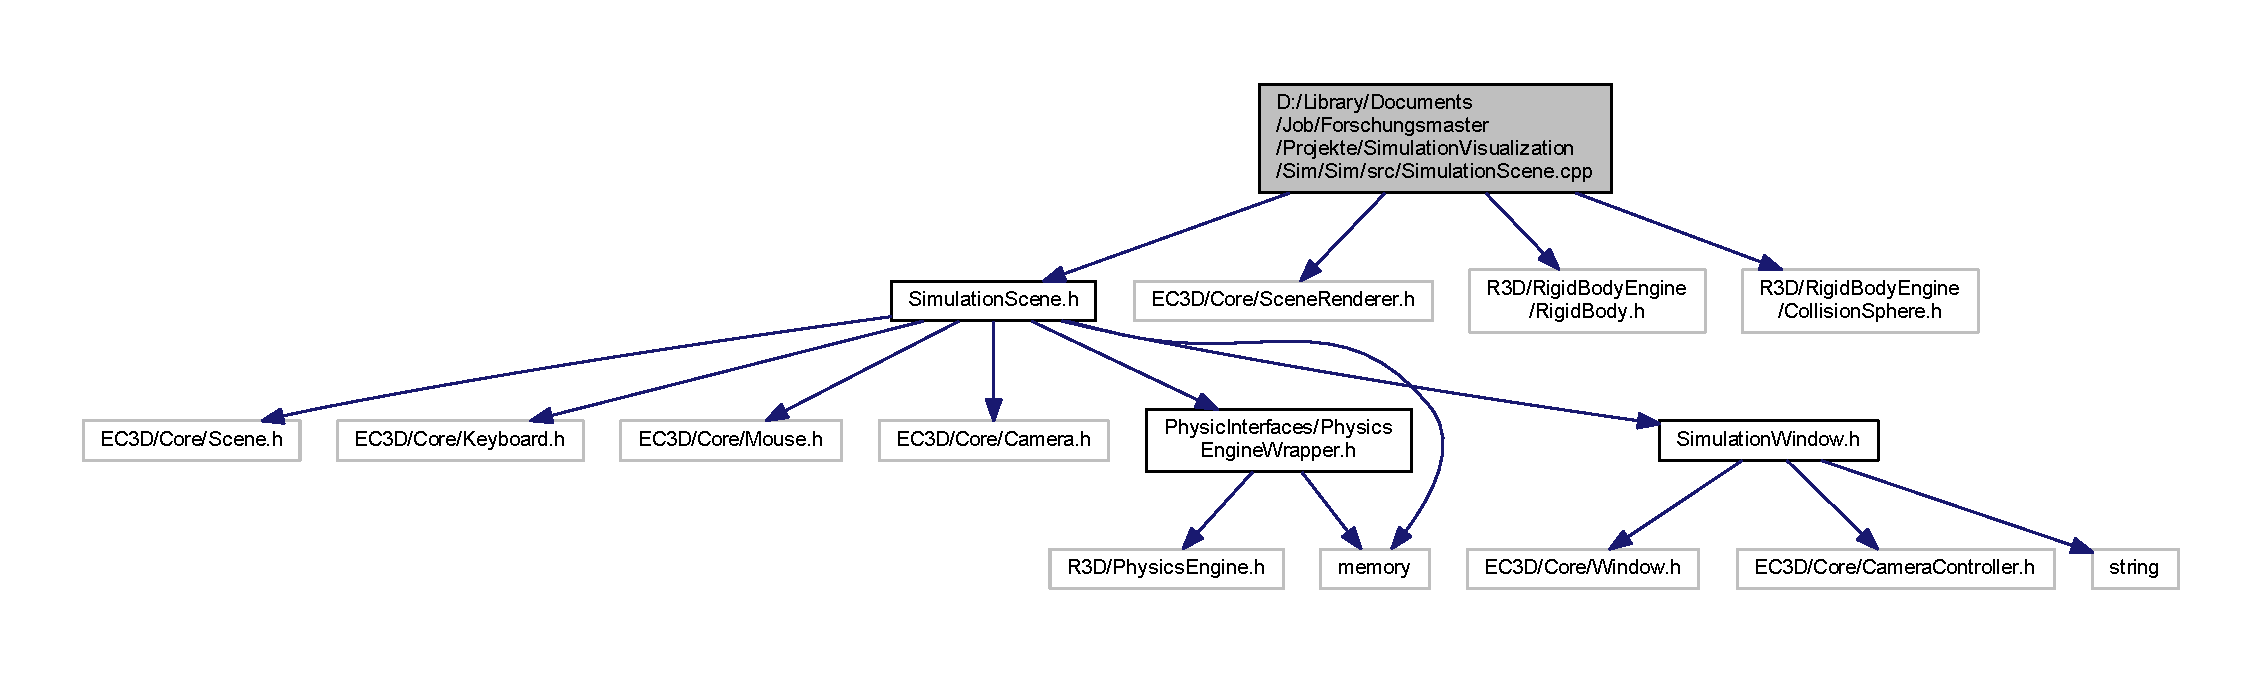
\includegraphics[width=350pt]{_simulation_scene_8cpp__incl}
\end{center}
\end{figure}

\hypertarget{_simulation_scene_8h}{}\section{D\+:/\+Library/\+Documents/\+Job/\+Forschungsmaster/\+Projekte/\+Simulation\+Visualization/\+Sim/\+Sim/src/\+Simulation\+Scene.h File Reference}
\label{_simulation_scene_8h}\index{D\+:/\+Library/\+Documents/\+Job/\+Forschungsmaster/\+Projekte/\+Simulation\+Visualization/\+Sim/\+Sim/src/\+Simulation\+Scene.\+h@{D\+:/\+Library/\+Documents/\+Job/\+Forschungsmaster/\+Projekte/\+Simulation\+Visualization/\+Sim/\+Sim/src/\+Simulation\+Scene.\+h}}
{\ttfamily \#include \char`\"{}E\+C3\+D/\+Core/\+Scene.\+h\char`\"{}}\newline
{\ttfamily \#include \char`\"{}E\+C3\+D/\+Core/\+Keyboard.\+h\char`\"{}}\newline
{\ttfamily \#include \char`\"{}E\+C3\+D/\+Core/\+Mouse.\+h\char`\"{}}\newline
{\ttfamily \#include \char`\"{}E\+C3\+D/\+Core/\+Camera.\+h\char`\"{}}\newline
{\ttfamily \#include \char`\"{}Physic\+Interfaces/\+Physics\+Engine\+Wrapper.\+h\char`\"{}}\newline
{\ttfamily \#include \char`\"{}Simulation\+Window.\+h\char`\"{}}\newline
{\ttfamily \#include $<$memory$>$}\newline
Include dependency graph for Simulation\+Scene.\+h\+:\nopagebreak
\begin{figure}[H]
\begin{center}
\leavevmode
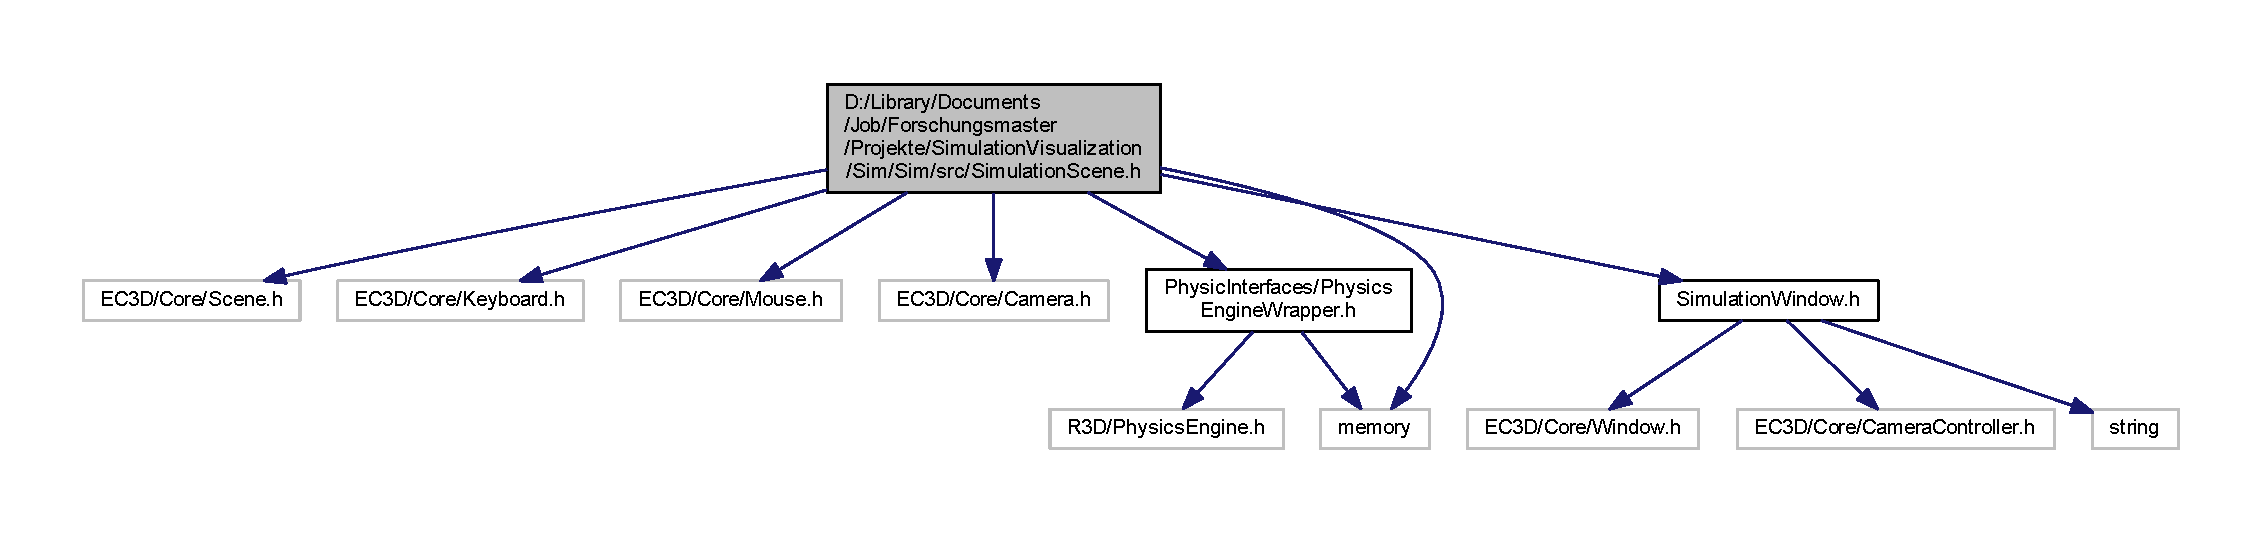
\includegraphics[width=350pt]{_simulation_scene_8h__incl}
\end{center}
\end{figure}
This graph shows which files directly or indirectly include this file\+:\nopagebreak
\begin{figure}[H]
\begin{center}
\leavevmode
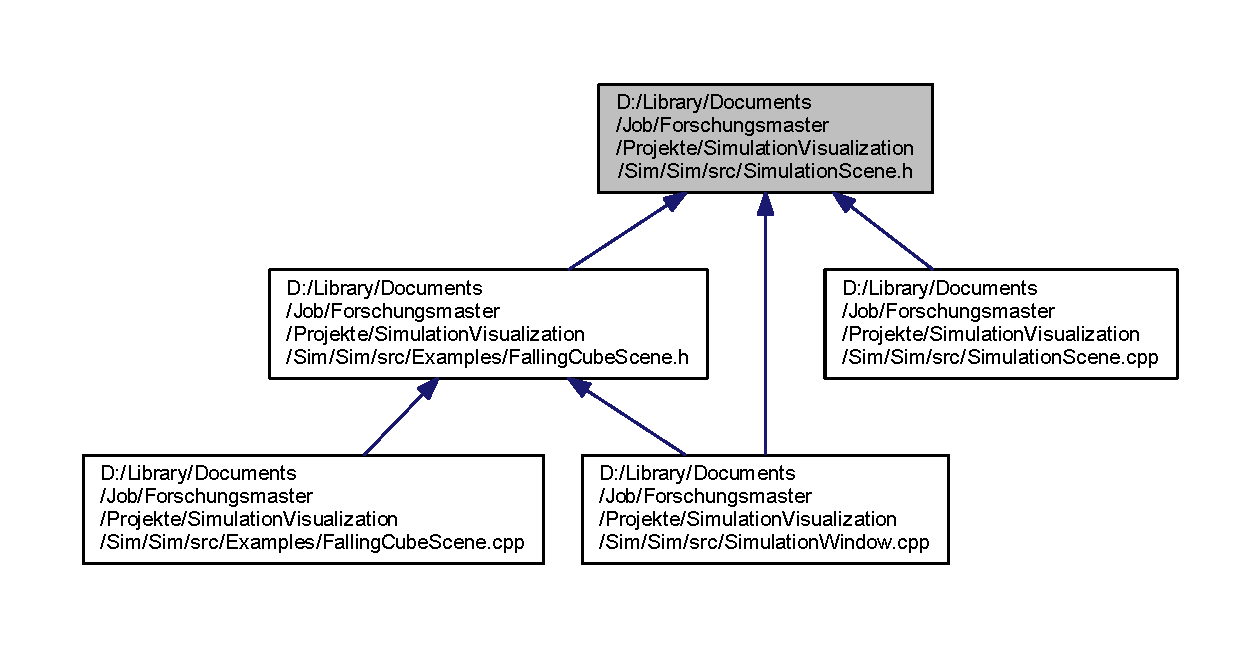
\includegraphics[width=350pt]{_simulation_scene_8h__dep__incl}
\end{center}
\end{figure}
\subsection*{Classes}
\begin{DoxyCompactItemize}
\item 
class \mbox{\hyperlink{class_simulation_scene}{Simulation\+Scene}}
\end{DoxyCompactItemize}
\subsection*{Namespaces}
\begin{DoxyCompactItemize}
\item 
 \mbox{\hyperlink{namespaceec}{ec}}
\end{DoxyCompactItemize}

\hypertarget{_simulation_window_8cpp}{}\section{D\+:/\+Library/\+Documents/\+Job/\+Forschungsmaster/\+Projekte/\+Simulation\+Visualization/\+Sim/\+Sim/src/\+Simulation\+Window.cpp File Reference}
\label{_simulation_window_8cpp}\index{D\+:/\+Library/\+Documents/\+Job/\+Forschungsmaster/\+Projekte/\+Simulation\+Visualization/\+Sim/\+Sim/src/\+Simulation\+Window.\+cpp@{D\+:/\+Library/\+Documents/\+Job/\+Forschungsmaster/\+Projekte/\+Simulation\+Visualization/\+Sim/\+Sim/src/\+Simulation\+Window.\+cpp}}
{\ttfamily \#include \char`\"{}Simulation\+Window.\+h\char`\"{}}\newline
{\ttfamily \#include \char`\"{}Simulation\+Scene.\+h\char`\"{}}\newline
{\ttfamily \#include \char`\"{}E\+C3\+D/\+Core/\+Cube\+Geometry.\+h\char`\"{}}\newline
{\ttfamily \#include \char`\"{}E\+C3\+D/\+Core/\+Sphere\+Geometry.\+h\char`\"{}}\newline
{\ttfamily \#include \char`\"{}E\+C3\+D/\+Core/\+Cylinder\+Geometry.\+h\char`\"{}}\newline
{\ttfamily \#include \char`\"{}E\+C3\+D/\+Core/\+Rectangle\+Geometry.\+h\char`\"{}}\newline
{\ttfamily \#include \char`\"{}E\+C3\+D/\+Core/\+Camera.\+h\char`\"{}}\newline
{\ttfamily \#include \char`\"{}E\+C3\+D/\+Core/\+Viewport.\+h\char`\"{}}\newline
{\ttfamily \#include \char`\"{}Examples/\+Falling\+Cube\+Scene.\+h\char`\"{}}\newline
Include dependency graph for Simulation\+Window.\+cpp\+:\nopagebreak
\begin{figure}[H]
\begin{center}
\leavevmode
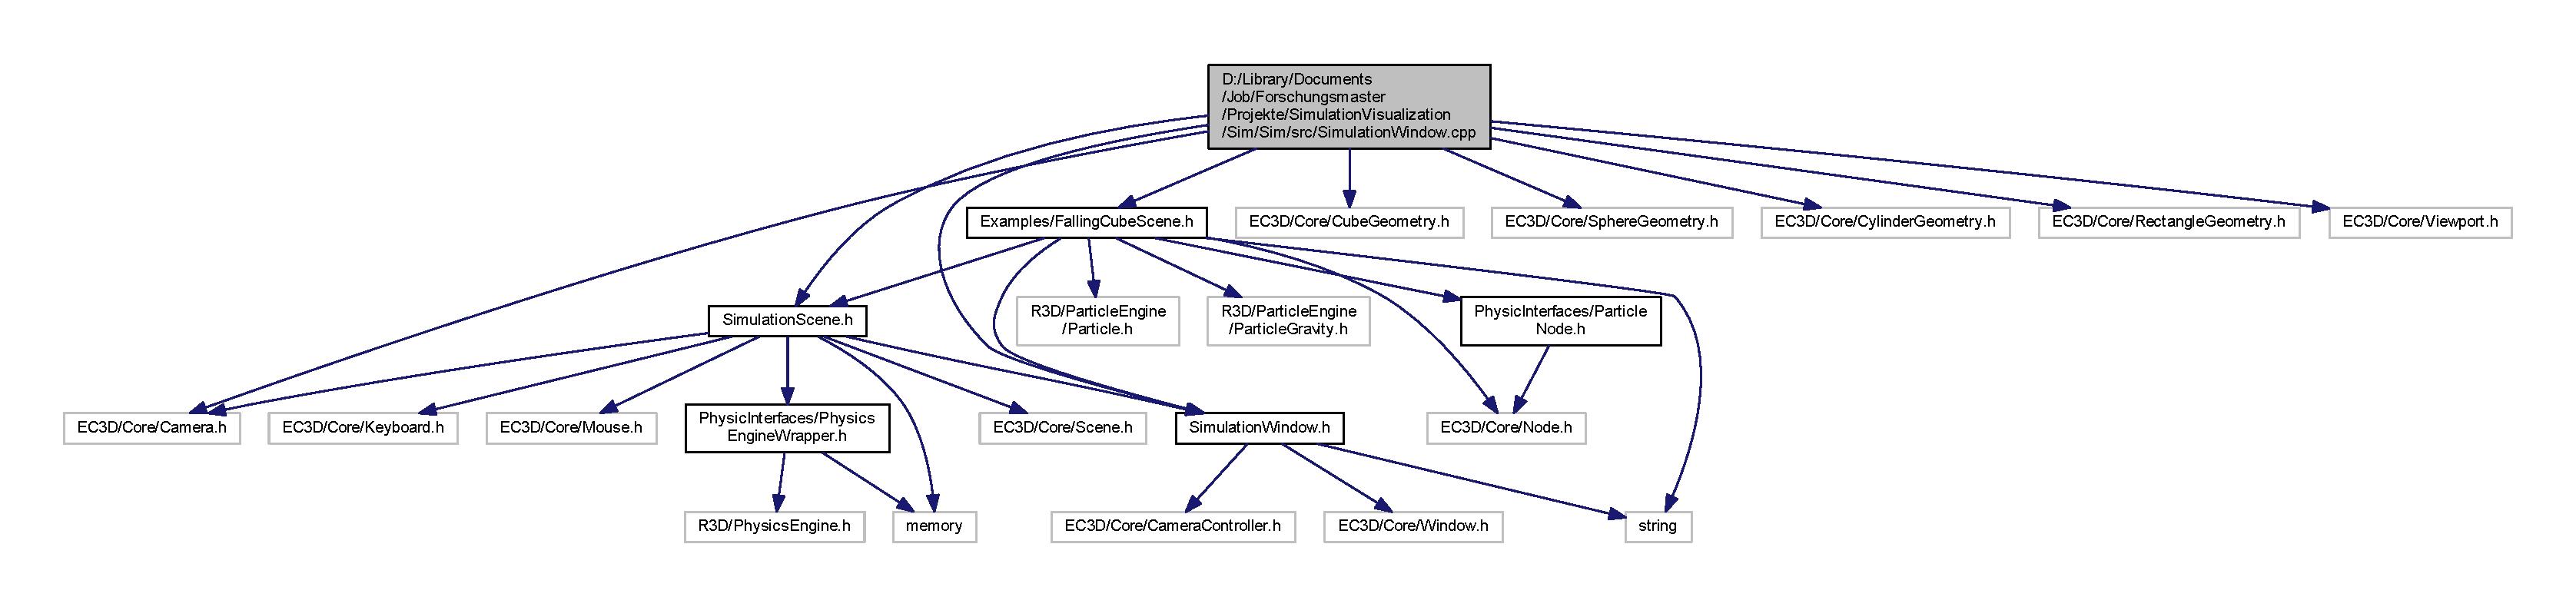
\includegraphics[width=350pt]{_simulation_window_8cpp__incl}
\end{center}
\end{figure}

\hypertarget{_simulation_window_8h}{}\section{D\+:/\+Library/\+Documents/\+Job/\+Forschungsmaster/\+Projekte/\+Simulation\+Visualization/\+Sim/\+Sim/src/\+Simulation\+Window.h File Reference}
\label{_simulation_window_8h}\index{D\+:/\+Library/\+Documents/\+Job/\+Forschungsmaster/\+Projekte/\+Simulation\+Visualization/\+Sim/\+Sim/src/\+Simulation\+Window.\+h@{D\+:/\+Library/\+Documents/\+Job/\+Forschungsmaster/\+Projekte/\+Simulation\+Visualization/\+Sim/\+Sim/src/\+Simulation\+Window.\+h}}
{\ttfamily \#include \char`\"{}E\+C3\+D/\+Core/\+Window.\+h\char`\"{}}\newline
{\ttfamily \#include \char`\"{}E\+C3\+D/\+Core/\+Camera\+Controller.\+h\char`\"{}}\newline
{\ttfamily \#include $<$string$>$}\newline
Include dependency graph for Simulation\+Window.\+h\+:\nopagebreak
\begin{figure}[H]
\begin{center}
\leavevmode
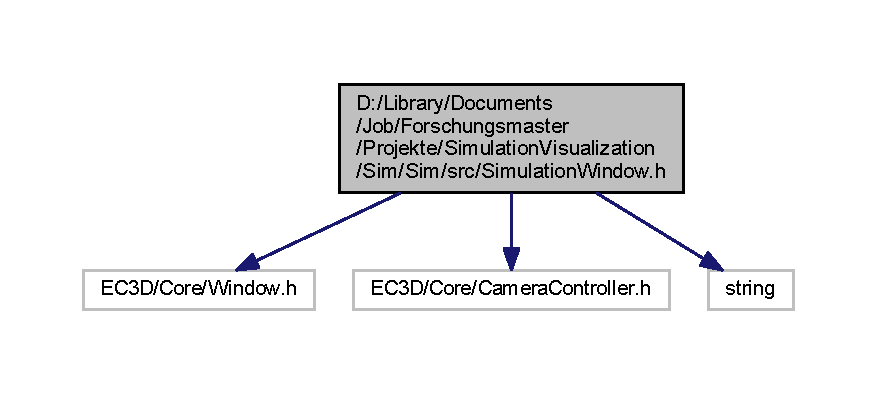
\includegraphics[width=350pt]{_simulation_window_8h__incl}
\end{center}
\end{figure}
This graph shows which files directly or indirectly include this file\+:\nopagebreak
\begin{figure}[H]
\begin{center}
\leavevmode
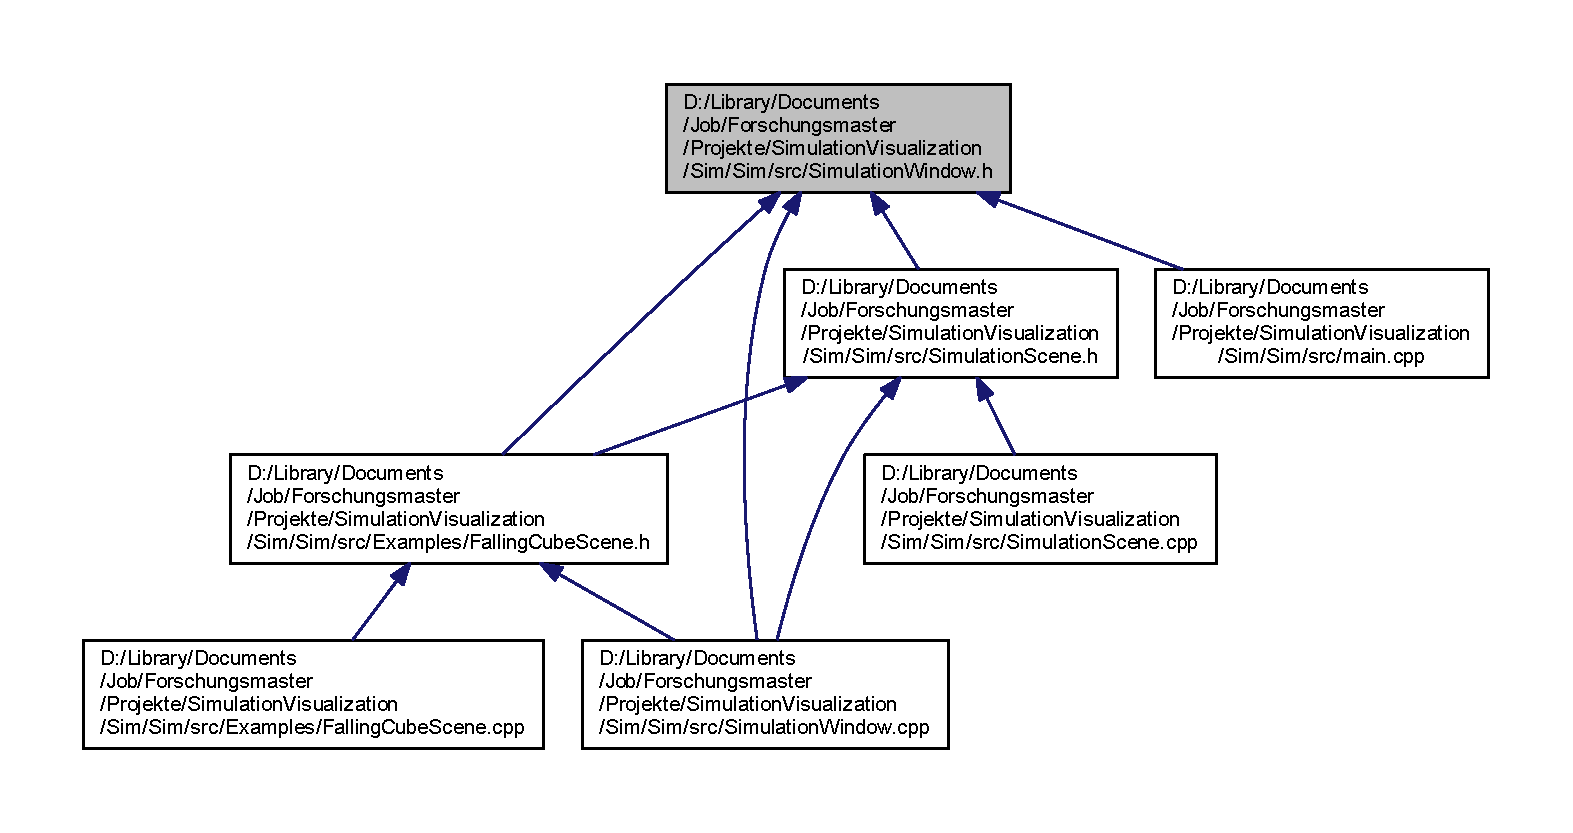
\includegraphics[width=350pt]{_simulation_window_8h__dep__incl}
\end{center}
\end{figure}
\subsection*{Classes}
\begin{DoxyCompactItemize}
\item 
class \mbox{\hyperlink{class_simulation_window}{Simulation\+Window}}
\end{DoxyCompactItemize}
\subsection*{Namespaces}
\begin{DoxyCompactItemize}
\item 
 \mbox{\hyperlink{namespaceec}{ec}}
\end{DoxyCompactItemize}

%--- End generated contents ---

% Index
\backmatter
\newpage
\phantomsection
\clearemptydoublepage
\addcontentsline{toc}{chapter}{Index}
\printindex

\end{document}
